%% ------------------------------------------------------------------------- %%
\chapter{Diagnóstico Bayesiano em Modelos de Regressão Assimétricos}
\label{cap:assimetrico}

A hipótese de simetria dos erros presente nos modelos apresentados no capítulo anterior pode não ser sempre adequada. Para analisar dados que não exibam simetria, nos últimos anos novos modelos têm sido propostos como alternativas aos modelos simétricos. O modelo de regressão $t$-assimétrico tem sido considerado uma alternativa robusta ao modelo normal \citep{Azzalini2008}.

Neste capítulo estudamos dois modelos que possuem erros com distribuição assimétrica: normal e $t$-Student. Os modelos normal assimétrico e $t$-assimétrico já foram estudados em \citet{Bayes2005:MSc} e \citet{Godoi2007:MSc}, respectivamente, e nestes trabalhos podemos encontrar formas de se obter estimativas dos parâmetros por meio da inferência bayesiana. Aqui complementamos o problema da estimação encontrando as condicionais completas do modelo $t$-assimétrico para uso do amostrador de Gibbs quando $\nu$ é considerado fixado.

A identificação das observações discrepantes também será feita por meio do cálculo do CPO para ambos modelos. Neste capítulo mostramos como obter estimativas para tal estatística. A medida de influência global e marginal também será por meio do cálculo das divergências norma $L_1$ e Kullback-Leibler e mostramos como obter estimativas destas medidas.

%% ------------------------------------------------------------------------- %%

\section{Modelo de Regressão Normal Assimétrico}
\label{sec:reg_normal_assim}


\subsection{Estimação dos Parâmetros}

O modelo de regressão linear com erros de distribuição normal assimétrica é dado por
\begin{equation}
y_i = x_i^\transp\betabf + \epsilon_i,
\end{equation}
onde, para cada $i=1,\ldots,n$, $y_i$ é a variável resposta da $i$-ésima observação, $x_i^\transp=(1,x_{i1},\ldots,x_{ip})$ é o vetor de variáveis explicativas, $\betabf=(\beta_0,\beta_1,\ldots,\beta_p)^\transp$ é vetor de parâmetros desconhecidos a serem estimados e $\epsilon_i\sim SN(0,\sigsq,\lambda)$ independentes, ou seja, os erros possuem distribuição normal assimétrica com posição $0$, escala $\sigsq$ e parâmetro de assimetria $\lambda$.

Neste caso, das propriedades da distribuição normal assimétrica, segue que $y_i\sim SN(x_i^\transp\betabf,\sigsq,\lambda)$ e sua função densidade de probabilidade é
\begin{equation}\label{eq:fdp_skewN}
f(y_i|\betabf,\sigsq,\lambda) = \frac{2}{\sigma}\phi\left(\frac{y_i-x_i^\transp\betabf}{\sigma}\right)\Phi\left(\lambda \frac{y_i-x_i^\transp\betabf}{\sigma}\right),
\end{equation}
onde $\phi$ e $\Phi$ são as funções densidade de probabilidade e distribuição acumulada de uma normal padrão, respectivamente. A esperança desta distribuição é dada por
\begin{equation}
E[y_i] = x_i^\transp\betabf + \sigma \sqrt{\frac{2}{\pi}}\frac{\lambda}{\sqrt{1+\lambda^2}},
\end{equation}
ou seja, a esperança da variável resposta não fica escrita originalmente como uma reta de regressão. Porém, ao considerarmos como intercepto
\begin{equation}
\beta_0^* = \beta_0 + \sigma \sqrt{\frac{2}{\pi}}\frac{\lambda}{\sqrt{1+\lambda^2}}
\end{equation}
teremos $E[y_i]=x_i^\transp\betabf^*$, com $\betabf^*=(\beta_0^*,\beta_1,\ldots,\beta_p)$.

Considere a seguinte representação hierárquica para cada $y_i$ apresentada em \citet{Bayes2005:MSc}
\begin{equation}
\begin{split}
y_i|v_i & \sim  N(x_i^\transp\betabf+\sigma\delta v_i,\sigma^2(1-\delta^2)) \\
v_i & \sim  HN(0,1),
\end{split}
\end{equation}
onde $\delta=\frac{\lambda}{\sqrt{1+\lambda^2}}$.

Sob a reparametrização $\eta=\sigma\delta$ e $\tau=\sigma\sqrt{1-\delta^2}$, reescrevemos o modelo como
\begin{equation}
\begin{split}
y_i|v_i & \sim N(x_i^\transp\betabf+\eta v_i,\tau^2) \\
v_i & \sim  HN(0,1),
\end{split}
\end{equation}
com $i=1,\ldots,n$.

Sob essa última parametrização a função de verossimilhança aumentada é dada por
\begin{equation}\label{eq:aug_ll_skewn}
L_A(\betabf,\tau,\eta) = \frac{1}{\tau^n} \exp\left(-\frac{1}{2\tausq}\sum_{i=1}^n(y_i-x_i^\transp\betabf - \eta v_i)^2\right)\exp\left(-\frac{1}{2}\sum_{i=1}^nv_i^2\right)\prod_{i=1}^n \mathbb{I}_{[0,\infty[}(v_i).
\end{equation}

Neste estudo, considerando desconhecimento prévio a respeito dos parâmetros a serem estimados, usamos distribuições \textit{a priori} não informativas. Dessa forma podemos considerar a seguinte distribuição \textit{a priori} de referência apresentada em \citet{Bayes2005:MSc} para $(\betabf,\sigma,\lambda)$
\begin{equation}
f(\betabf,\sigma,\lambda)\propto \frac{1}{\sigma}f(\lambda)
\end{equation}
com $\lambda \sim t(0,\sigma_t^2,k)$. Quando $k=\frac{1}{2}$ e $\sigma_t^2=\frac{\pi^2}{4}$ obtemos a aproximação da distribuição \textit{a priori} de Jeffreys e quando $k=2$ e $\sigma_t^2=\frac{1}{2}$ obtemos a distribuição \textit{a priori} induzida ao se considerar $\delta \sim U(]-1,1[)$. Para mais detalhes ver \citet{Bayes2005:MSc}.

Note que a distribuição $t$-Student pode ser representada de forma hierárquica como

\begin{equation}
\begin{split}
\lambda|\omega & \sim N\left(0,\frac{\sigma^2_t}{\omega}\right) \\
\omega & \sim Gama\left(\frac{k}{2},\frac{k}{2}\right).
\end{split}
\end{equation}
 
Consequentemente,
\begin{equation}
f(\betabf,\sigma,\lambda,\omega)\propto \frac{1}{\sigma}\exp\left(-\frac{\lambda^2\omega}{2\sigma_t^2}\right)\omega^{\frac{k+1}{2}-1}\exp\left(-\frac{k}{2}\omega\right).
\end{equation}

Como estamos trabalhando com a parametrização dada por $\eta=\sigma\delta$, $\tau=\sigma\sqrt{1-\delta^2}$ e $\delta=\lambda/\sqrt{1+\lambda^2}$, 
precisamos encontrar a distribuição \textit{a priori} $f(\betabf,\tau,\eta,\omega)$. Primeiramente, notemos que
\begin{equation}
f(\betabf,\tau,\eta,\omega) = f(\betabf)f(\tau,\eta|\omega)f(\omega)
\end{equation}
Logo, podemos considerar somente a seguinte transformação de variáveis aleatórias
\begin{equation}
(\sigma,\eta)|\omega\mapsto(\tau,\eta)|\omega=\left(\sigma\frac{1}{\sqrt{1+\lambda^2}},\sigma\frac{\lambda}{\sqrt{1+\lambda^2}}\right)|\omega
\end{equation}
e assim teremos
\begin{equation}
f(\tau,\eta|\omega)=f_{(\sigma,\lambda)|\omega}(\sqrt{\eta^2+\tau^2},\eta/\tau)\left|\frac{\partial(\sigma,\lambda)}{\partial(\tau,\eta)}\right|,
\end{equation}
onde $f_{(\sigma,\lambda)|\omega}$ é a função densidade de probabilidade conjunta de $(\sigma,\lambda)|\omega$ e 
\begin{equation}
\frac{\partial(\sigma,\lambda)}{\partial(\tau,\eta)}=
\begin{vmatrix}
\frac{\partial \sigma}{\partial \tau} & \frac{\partial \sigma}{\partial \eta} \\
\frac{\partial \lambda}{\partial \tau} & \frac{\partial \lambda}{\partial \eta}
\end{vmatrix}.
\end{equation}

Note que
\begin{equation}
\frac{\partial(\sigma,\lambda)}{\partial(\tau,\eta)}=
\begin{vmatrix}
\frac{\partial \sigma}{\partial \tau} & \frac{\partial \sigma}{\partial \eta} \\
\frac{\partial \lambda}{\partial \tau} & \frac{\partial \lambda}{\partial \eta}
\end{vmatrix}=
\begin{vmatrix}
\frac{\tau}{\sqrt{\eta^2+\tau^2}} & \frac{\eta}{\sqrt{\eta^2+\tau^2}}\\
-\frac{\eta}{\tau^2} & \frac{1}{\tau}
\end{vmatrix}=\frac{\sqrt{\eta^2+\tau^2}}{\tau^2}
\end{equation}
com
\begin{equation}
\begin{split}
f(\sigma)&\propto\frac{1}{\sigma}\\
\lambda|\omega & \sim N\left(0,\frac{\sigma^2_t}{\omega}\right).
\end{split}
\end{equation}

Logo,
\begin{equation}
\begin{split}
f(\tau,\eta|\omega)=&f_{(\sigma,\lambda)|\omega}(\sqrt{\eta^2+\tau^2},\eta/\tau)\left|\frac{\partial(\sigma,\lambda)}{\partial(\tau,\eta)}\right|=f_\sigma(\sqrt{\eta^2+\tau^2})f_{\lambda|\omega}(\eta/\tau|\omega)\frac{\sqrt{\eta^2+\tau^2}}{\tau^2} \\
\propto&\frac{1}{\sqrt{\eta^2+\tau^2}}\sqrt{\omega}\exp\left(-\frac{\eta^2\omega}{2\tau^2\sigma^2_t}\right)\frac{\sqrt{\eta^2+\tau^2}}{\tau^2}=\frac{\sqrt{\omega}}{\tau^2}\exp\left(-\frac{\eta^2\omega}{2\tau^2\sigma^2_t}\right)
\end{split}
\end{equation}
e, portanto,
\begin{equation}
\begin{split}\label{eq:prior_skewn}
f(\betabf,\tau,\eta,\omega)=&f(\betabf)f(\omega)f(\tau,\eta|\omega)\propto \omega^{\frac{k}{2}-1}\exp\left(-\frac{k}{2}\omega\right)\frac{\omega^\frac{1}{2}}{\tau^2}\exp\left(-\frac{\eta^2\omega}{2\tau^2\sigma^2_t}\right) \\
\propto&\frac{1}{\tau^2}\exp\left(-\frac{\eta^2\omega}{2\tau^2\sigma_t^2}\right)\omega^{\frac{k+1}{2}-1}\exp\left(-\frac{k}{2}\omega\right).
\end{split}
\end{equation}

A distribuição \textit{a posteriori} aumentada é dada por
\begin{equation}
\begin{split}\label{eq:post_aum_skewn}
f(\betabf,\tau,\eta,\omega,\vbf|\ybf)\propto & f(\ybf|\betabf,\tau,\eta,\omega,\vbf)f(\vbf)f(\betabf,\tau,\eta,\omega)=\\
=&L_A(\betabf,\tau,\eta)f(\betabf,\tau,\eta,\omega).
\end{split}
\end{equation}

A partir de \eqref{eq:aug_ll_skewn}, \eqref{eq:prior_skewn} e \eqref{eq:post_aum_skewn} conseguimos obtemos as distribuições condicionais completas apresentadas a seguir:
\begin{equation}
\begin{split}
\betabf|\tau,\eta,\omega,\vbf,\ybf & \sim N_{p+1}\left((X^\transp X)^{-1}X^\transp(Y-\eta V),\tau^2(X^\transp X)^{-1}\right) \\
\frac{1}{\tau^2}|\betabf,\eta,\omega,\vbf,\ybf & \sim Gama\left(\frac{n+1}{2},\frac{1}{2}\left((Y-\eta V-X\betabf)^\transp(Y-\eta V-X\betabf)+\frac{\eta^2\omega}{\sigma_t^2}\right)\right) \\
\eta|\betabf,\tau,\omega,\vbf,\ybf & \sim N\left(\frac{(Y-X\betabf)^\transp V}{V^\transp V+\frac{\omega}{\sigma_t^2}},\frac{\tau^2}{V^\transp V+\tfrac{\omega}{\sigma_t^2}}\right)\\
\omega|\betabf,\tau,\eta,\vbf,\ybf & \sim Gama\left(\frac{k+1}{2},\frac{1}{2}\left(k+\frac{\eta^2}{\tausq\sigma_t^2}\right)\right)\\
v_i|\betabf,\tau,\eta,\omega,\vbf,\ybf & \sim N\left(\frac{\eta(y_i-x_i^\transp\betabf)}{\eta^2+\tau^2},\frac{\tau^2}{\eta^2+\tau^2}\right)\mathbb{I}_{[0,\infty[}(v_i),\; i=1,\ldots,n
\end{split}
\end{equation}
onde
\begin{equation}
X=\begin{bmatrix}
1 & x_{11} & \cdots & x_{1p} \\
\vdots & \vdots & \ddots & \vdots \\
1 & x_{n1} & \cdots & x_{np}
\end{bmatrix},\;
Y=\begin{bmatrix}
y_1 \\
\vdots\\
y_n
\end{bmatrix},\;
V=\begin{bmatrix}
v_1 \\
\vdots\\
v_n
\end{bmatrix}
\end{equation}

Por meio das condicionais completas, podemos utilizar o amostrador de Gibbs para obter amostras das distribuições \textit{a posteriori} dos parâmetros e, daí, obter a inferência bayesiana para tais parâmetros. No apêndice apresentamos o programa que implementa este amostrador de Gibbs.

\subsection{Derivação das Medidas de Diagnóstico}
Considere $(\betabf^{(1)},{\sigsq}^{(1)},\lambda^{(1)}),\ldots,
(\betabf^{(L)},{\sigsq}^{(L)},\lambda^{(L)})$ uma amostra de tamanho $L$ simulada da distribuição \textit{a posteriori} conjunta. Esta amostra será utilizada em todos os cálculos das medidas de diagnóstico.

A estimativa para o $CPO_i$ no caso da regressão linear normal assimétrica será dada por
\begin{equation}\label{eq:cpo_est_sn}
\widehat{CPO_i} = \left[\frac{1}{L}\sum_{l=1}^L\frac{1}{f(y_i|\betabf^{(l)},{\sigsq}^{(l)},\lambda^{(l)})}\right]^{-1}
\end{equation}
onde $f(y_i|\betabf,\sigsq,\lambda)$ é a função de distribuição normal assimétrica de posição $x_i^\transp\betabf$, escala $\sigsq$ e assimetria $\lambda$.

A estimativa da divergência para a influência global é dada por
\begin{equation}
\widehat{D_{\betabf,\sigsq,\lambda}(g,i)} = \frac{1}{L}\sum_{l=1}^L g\left(\frac{\widehat{CPO_i}}{f(y_i|\betabf^{(l)},{\sigsq}^{(l)},\lambda^{(l)})}\right)
\end{equation}
onde $\widehat{CPO_i}$ é a estimativa para o $CPO_i$ obtida em \eqref{eq:cpo_est_sn}. Para a obtenção da norma $L_1$ e da divergência Kullback-Leibler basta substituir a função $g$ adequada para cada caso.

\begin{prop}
Uma estimativa de Monte Carlo da divergência para a influência marginal no modelo normal assimétrico é dada por
\begin{equation}
\widehat{D_\betabf(g,i)} = \frac{1}{L}\sum_{l=1}^L g\left(\frac{\widehat{CPO_i}}{\hat{f}(y_i|\betabf^{(l)},\yi)}\right)
\end{equation}
onde $\widehat{CPO_i}$ é a estimativa para o $CPO_i$ obtida em \eqref{eq:cpo_est_t} e 
\begin{equation}
\begin{split}
\hat{f}(y_i|\betabf,\yi) =
\frac{\Gamma(\frac{n-1}{2})\frac{1}{M}\sum_{m=1}^M\left[(\Omega_{(m)}+V_{(m)}) A_{(m)}^{n-1}\right]^{-\frac{1}{2}}}
{\Gamma(\frac{n-2}{2})\sqrt{\pi}\frac{1}{M}\sum_{m=1}^M \left[ \left(\Omega_{(m)} + \sum_{k \neq i}{v_k^{(m)}}^2\right) K_{(m)}^{n-2}\right]^{-\frac{1}{2}}}
\end{split}
\end{equation}
com
\begin{equation}
\begin{split}
z_i & = y_i - x_i^\transp\betabf \\
A_{(m)} & = \sum_{j=1}^nz_j^2 - \frac{1}{\Omega_{(m)} + V_{(m)}}\left(\sum_{k=1}^nv_k^{(m)}z_k\right)^2 \\
K_{(m)} & = \sum_{j\neq i}z_j^2-\frac{1}{\Omega_{(m)}+\sum_{k \neq i}{v_k^{(m)}}^2}\left(\sum_{j\neq i}v_j^{(m)}z_j\right)^2 \\
V_{(m)} & = \sum_{j=1}^n {v_j^{(m)}}^2 \\
\Omega_{(m)} & = \frac{\omega_{(m)}}{\sigsq_t}
\end{split}
\end{equation}
onde, para cada $j=1,\ldots,n$, $v_j^{(1)},\ldots,v_j^{(M)}$ são valores simulados independentes da distribuição $HN(0,1)$ e $\omega^{(1)},\ldots,\omega^{(M)}$ são valores simulados da distribuição $Gama((k+1)/2,k/2)$.
\end{prop}

\begin{proof}
Primeiro, vamos obter uma expressão para $f(y_i|\betabf,\yi)$. Segue de \eqref{eq:fyi_perturb} que: 
\begin{align}\label{eq:sn_marg_1}
f(y_i|\betabf,\yi) & \propto \int\int\int f(\ybf|\betabf,\tausq,\eta,\omega) f(\betabf,\tausq,\eta,\omega) d\tausq d\eta d\omega \notag \\
 {} &= \int\int\int \int f(\ybf|\betabf,\tausq,\eta,\omega,\vbf)f(\vbf|\betabf,\tausq,\eta,\omega) d\vbf f(\betabf,\tausq,\eta,\omega)  d\tausq d\eta d\omega \notag \\
 {} &= \int\int\int \int f(\ybf|\betabf,\tausq,\eta,\omega,\vbf)f(\vbf) f(\betabf,\tausq,\eta,\omega) d\vbf d\tausq d\eta d\omega \notag \\
{}&\propto \int\int\int \int f(\ybf|\betabf,\tausq,\eta,\omega,\vbf)\frac{1}{\tausq}f(\vbf)f(\eta|\omega)g(\omega) d\vbf d\tausq d\eta d\omega  \notag \\
{}& \propto \int\int\int \int \frac{1}{\tau^n}\exp\left(\frac{-1}{2\tausq}\sum_{j=1}^n(y_j-x_j^\transp\betabf - \eta v_j)^2\right)\frac{1}{\tausq}f(\vbf) \notag \\
{}& \qquad \exp\left(\frac{-\eta^2\omega}{2\tausq\sigsq_t}\right)g(\omega)d\vbf d\tausq d\eta d\omega \notag \\
{}& \propto \int\int\int \int \frac{1}{\tau^{n+2}}\exp\left(\frac{-1}{2\tausq}\left(\sum_{j=1}^n(y_j-x_j^\transp\betabf - \eta v_j)^2+\frac{\omega\eta^2}{\sigsq_t}\right)\right)  d\tausq  \notag \\
{}& \qquad f(\vbf)g(\omega)d\vbf d\eta d\omega  \notag \\
{}& \propto  \int\int\int \left[\sum_{j=1}^n(y_j-x_j^\transp\betabf - \eta v_j)^2+\frac{\omega\eta^2}{\sigsq_t}\right]^{-\frac{n}{2}} d\eta f(\vbf)g(\omega)d\vbf d\omega
\end{align}
onde $f(\vbf)$ é a função densidade de probabilidade de $\vbf=(v_1,\ldots,v_n)$, com $v_i\sim HN(0,1)$, $i=1,\ldots,n$, e $g(\omega)$ é a função densidade de probabilidade de $\omega\sim Gama(\frac{k+1}{2},\frac{k}{2})$.

Fazendo $\xi = \frac{\sum_{j=1}^nv_j(y_j-x_j^\transp\betabf)}{\sum_{j=1}^nv_j^2}$ para isolar $\eta$ em \eqref{eq:sn_marg_1} teremos
\begin{align}\label{eq:sn_marg_2}
& \sum_{j=1}^n(y_j-x_j^\transp\betabf - \eta v_j)^2+\frac{\omega\eta^2}{\sigsq_t} \notag \\
& =  \sum_{j=1}^nv_j^2\left(\frac{y_j-x_j^\transp\betabf}{v_j} - \xi\right)^2+\sum_{j=1}^nv_j^2(\xi-\eta)^2+\frac{\omega\eta^2}{\sigsq_t} \notag \\
{} & =  \sum_{j=1}^nv_j^2\left(\frac{y_j-x_j^\transp\betabf}{v_j} - \xi\right)^2 +\notag \\
{}&\quad+\left(\sum_{j=1}^nv_j^2+\frac{\omega}{\sigsq_t}\right)\left(\eta-\frac{\sum_{j=1}^nv_j^2\xi}{\sum_{j=1}^nv_j^2+\frac{\omega}{\sigsq_t}}\right)^2+\frac{\sum_{j=1}^nv_j^2\frac{\omega}{\sigsq_t}\xi^2}{\sum_{j=1}^nv_j^2+\frac{\omega}{\sigsq_t}}  \notag \\
{} & =  \underbrace{\sum_{j=1}^nv_j^2\left(\frac{y_j-x_j^\transp\betabf}{v_j} - \xi\right)^2 +\frac{\sum_{j=1}^nv_j^2\frac{\omega}{\sigsq_t}\xi^2}{\sum_{j=1}^nv_j^2+\frac{\omega}{\sigsq_t}}}_{A} + \notag \\
{}& \quad  + \left(\underbrace{\sum_{j=1}^nv_j^2+\frac{\omega}{\sigsq_t}}_{B}\right)\left(\eta-\underbrace{\frac{\sum_{j=1}^nv_j^2\xi}{\sum_{j=1}^nv_j^2+\frac{\omega}{\sigsq_t}}}_{C}\right)^2 \notag \\
{} & = A + B(\eta - C)^2.
\end{align}

Veja que podemos buscar agora uma forma para o resultado de \eqref{eq:sn_marg_2} que envolva uma distribuição de probabilidade conhecida em $\eta$

\begin{equation}\label{eq:sn_marg_3}
\begin{split}
\left[A + B(\eta - C)^2\right]^{-\frac{n}{2}} & = A^{-\frac{n}{2}}\left[1 + \frac{B}{A}(\eta - C)^2\right]^{-\frac{n}{2}} \\
{} & = A^{-\frac{n}{2}}\left[1 + \left(\frac{\eta - C}{\sqrt{A}/\sqrt{B}}\right)^2\right]^{-\frac{n}{2}} \\
{} & = A^{-\frac{n}{2}}\left[1 + \frac{1}{n-1}\left(\frac{\eta - C}{\sqrt{A}/\sqrt{(n-1)B}}\right)^2\right]^{-\frac{n}{2}} \\
{} & = A^{-\frac{n}{2}}h^*(\eta),
\end{split}
\end{equation}
onde $h^*$ é o núcleo de uma distribuição $t(C,\sqrt{A}/\sqrt{(n-1)B},n-1)$. Logo, podemos continuar o cálculo de \eqref{eq:sn_marg_1} com o resultado encontrado em \eqref{eq:sn_marg_3}. Assim
\begin{equation}\label{eq:sn_marg_4}
\begin{split}
f(y_i|\betabf,\yi)  & \propto  \int\int\int\left[\sum_{j=1}^n(y_j-x_j^\transp\betabf - \eta v_j)^2+\frac{\omega\eta^2}{\sigsq_t}\right]^{-\frac{n}{2}} d\eta f(\vbf)g(\omega)d\vbf d\omega \\
{} & = \int\int\int A^{-\frac{n}{2}}h^*(\eta) d\eta f(\vbf)g(\omega)d\vbf d\omega \\
{} & = \int\int A^{-\frac{n}{2}}\left[\int h^*(\eta) d\eta\right] f(\vbf)g(\omega)d\vbf d\omega\\
{} & = \int\int A^{-\frac{n}{2}}\frac{\Gamma\left(\frac{n-1}{2}\right)\sqrt{\pi A}}{\Gamma\left(\frac{n}{2}\right)\sqrt{B}} f(\vbf)g(\omega)d\vbf d\omega \\
{} & \propto \int\int A^{-\frac{n-1}{2}}B^{-\frac{1}{2}}f(\vbf)g(\omega)d\vbf d\omega.
\end{split}
\end{equation}

Note que na equação \eqref{eq:sn_marg_4} obtivemos um resultado proporcional para $f(y_i|\betabf,\yi)$, iremos agora calcular a constante de normalização. Dessa forma,
\begin{equation}\label{eq:sn_marg_5}
\int \int\int A^{-\frac{n-1}{2}}B^{-\frac{1}{2}}f(\vbf)g(\omega)d\vbf d\omega d y_i  =  \int\int B^{-\frac{1}{2}}\left[ \int A^{-\frac{n-1}{2}}d y_i \right]f(\vbf)g(\omega)d\vbf d\omega 
\end{equation}
com $A=\sum_{j=1}^nv_j^2\left(\frac{y_j-x_j^\transp\betabf}{v_j} - \xi\right)^2 + \frac{\sum_{j=1}^nv_j^2\frac{\omega}{\sigsq_t}\xi^2}{\sum_{j=1}^nv_j^2+\frac{\omega}{\sigsq_t}}$, $\xi = \frac{\sum_{j=1}^nv_j(y_j-x_j^\transp\betabf)}{\sum_{j=1}^nv_j^2}$ e $ B = \sum_{j=1}^nv_j^2+\frac{\omega}{\sigsq_t}$.

Integrando em $y_i$, temos
\begin{equation}\label{eq:sn_marg_6}
\begin{split}
\int A^{-\frac{n-1}{2}} d y_i = \int \left[\sum_{j=1}^nv_j^2\left(\frac{y_j-x_j^\transp\betabf}{v_j} - \xi\right)^2 + \frac{\sum_{j=1}^nv_j^2\frac{\omega}{\sigsq_t}\xi^2}{\sum_{j=1}^nv_j^2+\frac{\omega}{\sigsq_t}}\right]^{-\frac{n-1}{2}}d y_i
\end{split}
\end{equation}

Podemos trabalhar melhor a fórmula que está sendo integrada deixando o termo $y_i$ em maior evidência. Assim teremos

\begin{equation}
\begin{split}
& \sum_{j=1}^nv_j^2\left(\frac{y_j-x_j^\transp\betabf}{v_j} - \xi\right)^2 + \frac{\sum_{j=1}^nv_j^2\frac{\omega}{\sigsq_t}\xi^2}{\sum_{j=1}^nv_j^2+\frac{\omega}{\sigsq_t}} \\
& = \sum_{j=1}^nv_j^2\left(\frac{y_j-x_j^\transp\betabf}{v_j} - \frac{\sum_{k=1}^nv_k(y_k-x_k^\transp\betabf)}{\sum_{k=1}^nv_k^2}\right)^2 + \frac{\sum_{j=1}^nv_j^2\frac{\omega}{\sigsq_t}\left(\frac{\sum_{k=1}^nv_k(y_k-x_k^\transp\betabf)}{\sum_{k=1}^nv_k^2}\right)^2}{\sum_{j=1}^nv_j^2+\frac{\omega}{\sigsq_t}}.
\end{split}
\end{equation}

Para simplificar a notação, considere $\Omega = \frac{\omega}{\sigsq_t}$, $V = \sum_{k=1}^nv_k^2$ e $z_j = y_j - x_t^\transp\betabf$. Assim
\begin{equation}\label{eq:sn_marg_8}
\begin{split}
\sum_{j=1}^nv_j^2\left(\frac{y_j-x_j^\transp\betabf}{v_j} - \xi\right)^2 + \frac{\sum_{j=1}^nv_j^2\frac{\omega}{\sigsq_t}\xi^2}{\sum_{j=1}^nv_j^2+\frac{\omega}{\sigsq_t}}  &= \sum_{j=1}^n\left(z_j - v_j\frac{\sum_{k=1}^nv_kz_k}{V}\right)^2 + \frac{V \Omega \left(\frac{\sum_{k=1}^nv_kz_k}{V}\right)^2}{\Omega + V} \\
{} & =\underbrace{\sum_{j=1}^n\left(z_j - \frac{v_j}{V}\sum_{k=1}^nv_kz_k\right)^2}_{(*)} + \underbrace{\frac{\Omega/V}{\Omega + V}  \left(\sum_{k=1}^nv_kz_k\right)^2}_{(**)}.
\end{split}
\end{equation}

Vamos trabalhar agora com uma das parcelas da soma resultante na equação \eqref{eq:sn_marg_8}, denotadas por $(*)$ e $(**)$, de forma separada. Para a primeira parcela da soma temos
\begin{equation}
\begin{split}
(*)& =\sum_{j=1}^n\left(z_j - \frac{v_j}{V}\sum_{k=1}^nv_kz_k\right)^2  = \sum_{j=1}^n\left(z_j^2+\frac{v_j^2}{V^2}\left(\sum_{k=1}^nv_kz_k\right)^2-\frac{2v_jz_j}{V}\sum_{k=1}^nv_kz_k\right) \\
{} & = \sum_{j=1}^nz_j^2 +\frac{\left(\sum_{k=1}^nv_kz_k\right)^2}{V^2}\sum_{j=1}^nv_j^2 -\frac{2\sum_{k=1}^nv_kz_k}{V}\sum_{j=1}^nv_jz_j  \\
{} & = \sum_{j=1}^nz_j^2 +\frac{\left(\sum_{k=1}^nv_kz_k\right)^2}{V} -\frac{2\left(\sum_{k=1}^nv_kz_k\right)^2}{V} \\
{} & = \sum_{j=1}^nz_j^2 -\frac{1}{V}\left(\sum_{k=1}^nv_kz_k\right)^2.
\end{split}
\end{equation}

Dessa forma, a soma completa será dada por
\begin{align}\label{eq:sn_marg_10}
(*)+(**) & = \sum_{j=1}^nz_j^2 -\frac{1}{V}\left(\sum_{k=1}^nv_kz_k\right)^2  + \frac{\Omega}{\Omega + V}\frac{1}{V}  \left(\sum_{k=1}^nv_kz_k\right)^2 \notag \\
{} & = \sum_{j=1}^nz_j^2 + \frac{1}{V}\left(\sum_{k=1}^nv_kz_k\right)^2\left(\frac{\Omega}{\Omega + V} - 1\right) \notag \\
{} & = \sum_{j=1}^nz_j^2 - \frac{1}{\Omega + V}\left(\sum_{k=1}^nv_kz_k\right)^2 \notag \\
{} & = z_i^2 + \sum_{j\neq i}z_j^2 - \frac{1}{\Omega + V}\left(v_iz_i + \sum_{k\neq i} v_kz_k\right)^2 \notag \\
{} & = z_i^2 + \sum_{j\neq i}z_j^2 - \frac{1}{\Omega + V}\left(v_i^2z_i^2 + \left(\sum_{k\neq i} v_kz_k\right)^2 +2v_iz_i\sum_{k\neq i} v_kz_k\right) \notag \\
{} & = z_i^2\left[1-\frac{v_i^2}{\Omega + V}\right] + z_i\left[-\frac{2v_i}{\Omega + V}\sum_{k\neq i} v_kz_k\right] + \sum_{j\neq i}z_j^2 - \frac{1}{\Omega + V}\left(\sum_{k\neq i} v_kz_k\right)^2 \notag \\
{} & = D(z_i - H)^2+K
\end{align}
para $D$, $H$ e $K$ convenientes, pois no penúltimo passo da equação \eqref{eq:sn_marg_10} temos um polinômio de segundo grau em $z_i$. Logo, retomando o cálculo da equação \eqref{eq:sn_marg_6},
\begin{equation}\label{eq:sn_marg_11}
\begin{split}
& \int \left[\sum_{j=1}^nv_j^2\left(\frac{y_j-x_j^\transp\betabf}{v_j} - \xi\right)^2 + \frac{\sum_{j=1}^nv_j^2\frac{\omega}{\sigsq_t}\xi^2}{\sum_{j=1}^nv_j^2+\frac{\omega}{\sigsq_t}}\right]^{-\frac{n-1}{2}}dy_i \\
& = \int\left[D(z_i - H)^2+K\right]^{-\frac{n-1}{2}} dy_i \\
& = \int\left[D(y_i - x_i^\transp\betabf - H)^2+K\right]^{-\frac{n-1}{2}} dy_i\\
& = K^{-\frac{n-1}{2}}\int\left[1+\frac{1}{n}\left(\frac{y_i-x_i^\transp\betabf-H}{\sqrt{K}/\sqrt{nD}}\right)^2\right]^{-\frac{n-1}{2}}dy_i \\
& = \frac{\Gamma\left(\frac{n-2}{2}\right)\sqrt{\pi}}{\Gamma\left(\frac{n-1}{2}\right)}\frac{K^{-\frac{n-2}{2}}}{\sqrt{D}}.
\end{split}
\end{equation}

Com os resultados obtidos nas equações \eqref{eq:sn_marg_4} e \eqref{eq:sn_marg_11} conseguimos calcular $f(y_i|\betabf,\yi)$ por meio da seguinte equação
\begin{equation}\label{eq:sn_marg_12}
\begin{split}
f(y_i|\betabf,\yi) = \frac{
\Gamma\left(\frac{n-1}{2}\right)\int B^{-\frac{1}{2}} A^{-\frac{n-1}{2}}f(\vbf)g(\omega)d\vbf d\omega
}{
\Gamma\left(\frac{n-2}{2}\right) \sqrt{\pi}\int B^{-\frac{1}{2}}D^{-\frac{1}{2}} K^{-\frac{n-2}{2}}f(\vbf)g(\omega)d\vbf d\omega 
} \\
{} = \frac{
\Gamma\left(\frac{n-1}{2}\right)\int \left[(\Omega+V) A^{n-1}\right]^{-\frac{1}{2}}f(\vbf)g(\omega)d\vbf d\omega
}{
\Gamma\left(\frac{n-2}{2}\right) \sqrt{\pi}\int \left[ (\Omega + \sum_{k \neq i}v_k^2) K^{n-2}\right]^{-\frac{1}{2}}f(\vbf)g(\omega)d\vbf d\omega 
}
\end{split}
\end{equation}
com 
\begin{align}
z_i & = y_i - x_i^\transp\betabf \notag ,\\
\Omega & = \frac{\omega}{\sigsq_t} \notag ,\\
V & = \sum_{k=1}^nv_k^2 \notag ,\\
D & = 1-\frac{v_i^2}{\Omega+V} \notag ,\\
K & = \sum_{j\neq i}z_j^2-\frac{1}{\Omega+\sum_{k \neq i}v_k^2}\left(\sum_{j\neq i}v_jz_j\right)^2  ,\\
B & = \sum_{j=1}^nv_j^2+\frac{\omega}{\sigsq_t} \notag ,\\
A & = \sum_{j=1}^nz_j^2 - \frac{1}{\Omega + V}\left(\sum_{k=1}^nv_kz_k\right)^2 \notag .
\end{align}

Com o resultado obtido na equação \eqref{eq:sn_marg_12}, via integração de Monte Carlo, podemos calcular de forma aproximada $f(y_i|\betabf,\yi)$. Seja $\vbf^{(m)} = (v_1^{(m)},\ldots,v_n^{(m)})$, $l=1,\ldots,M$, tal que $v_i^{(m)}$ é uma amostra de $v_i\sim HN(0,1)$ e $\omega^{(m)}$, $l=1,\ldots,M$, uma amostra de $\omega \sim Gama((k+1)/2,k/2)$, então
\begin{equation}
\begin{split}
\hat{f}(y_i|\betabf,\yi) =
\frac{\Gamma(\frac{n-1}{2})\frac{1}{M}\sum_{m=1}^M\left[(\Omega_{(m)}+V_{(m)}) A_{(m)}^{n-1}\right]^{-\frac{1}{2}}}
{\Gamma(\frac{n-2}{2})\sqrt{\pi}\frac{1}{M}\sum_{m=1}^M \left[ \left(\Omega_{(m)} + \sum_{k \neq i}{v_k^{(m)}}^2\right) K_{(m)}^{n-2}\right]^{-\frac{1}{2}}}
\end{split}
\end{equation}
com
\begin{equation}
\begin{split}
z_i & = y_i - x_i^\transp\betabf, \\
A_{(m)} & = \sum_{j=1}^nz_j^2 - \frac{1}{\Omega_{(m)} + V_{(m)}}\left(\sum_{k=1}^nv_k^{(m)}z_k\right)^2 ,\\
K_{(m)} & = \sum_{j\neq i}z_j^2-\frac{1}{\Omega_{(m)}+\sum_{k \neq i}{v_k^{(m)}}^2}\left(\sum_{j\neq i}v_j^{(m)}z_j\right)^2 ,\\
V_{(m)} & = \sum_{j=1}^n {v_j^{(m)}}^2 ,\\
\Omega_{(m)} & = \frac{\omega_{(m)}}{\sigsq_t}.
\end{split}
\end{equation}

\end{proof}

\section{Modelo de Regressão $t$-Student Assimétrico}
\label{sec:reg_t_assim}

\subsection{Estimação dos Parâmetros}

O modelo de regressão linear com resposta de distribuição $t$-assimétrica é dado por
\begin{equation} \label{eq:modelo_skew_t}
y_i = x_i^\transp\betabf + \epsilon_i,
\end{equation}
onde, para cada $i=1,\ldots,n$, $y_i$ é a variável resposta da observação $i$, $x_i^\transp=(1,x_{i1},\ldots,x_{ip})$ é o vetor de variáveis explicativas, $\betabf=(\beta_0,\beta_1,\ldots,\beta_p)^\transp$ é vetor de parâmetros desconhecidos a serem estimados e $\epsilon_i\sim ST(0,\sigma,\nu,\lambda)$, ou seja, os erros possuem distribuição $t$-assimétrica com parâmetro de posição $0$, escala $\sigma$, graus de liberdade $\nu$ (fixado) e assimetria $\lambda$.

Note que para cada $i$, pelas propriedades da distribuição $t$-assimétrica, temos que $y_i\sim ST(x_i^\transp\betabf,\sigma,\nu,\lambda)$, cuja função densidade de probabilidade é
\begin{equation}
f(y_i|\betabf,\sigsq,\lambda) = \frac{2}{\sigma}t_\nu\left(\frac{y_i-x_i^\transp\betabf}{\sigma}\right)T_{\nu+1}\left(\lambda \frac{y_i-x_i^\transp\betabf}{\sigma}\sqrt{\frac{\nu+1}{\nu+\sigma^{-2}(y_i-x_i^\transp\betabf)^2}}\right),
\end{equation}
com $t_\gamma$ e $T_\gamma$ as funções densidade de probabilidade e de distribuição de uma $t$-Student padrão com $\gamma$ graus de liberdade. De forma análoga ao caso normal assimétrico, se quisermos que a esperança de $y_i$ seja escrita como uma reta de regressão precisamos considerar o seguinte intercepto
\begin{equation}
\beta_0^*=\beta_0 + \sigma \sqrt{\frac{\nu}{\pi}} \frac{\lambda}{\sqrt{1+\lambda^2}}\frac{\Gamma\left(\frac{\nu-1}{2}\right)}{\left(\frac{\nu}{2}\right)}
\end{equation}
e, assim, $E[y_i]=x_i^\transp\betabf^*$, com $\betabf^*=(\beta_0^*,\beta_1,\ldots,\beta_p)$.

Podemos utilizar a seguinte representação hierárquica, dada em \citet{Godoi2007:MSc}, para cada $y_i$
\begin{equation} \label{eq:forma_hier}
\begin{split}
y_i|u_i,v_i & \sim  N\left(x_i^\transp\betabf+\sigma\delta\frac{v_i}{\sqrt{u_i}},\frac{\sigma^2(1-\delta^2)}{u_i}\right) \\
u_i & \sim  Gama\left(\frac{\nu}{2},\frac{\nu}{2}\right) \\
v_i & \sim  HN(0,1),
\end{split}
\end{equation}
onde $\delta=\lambda/(\sqrt{1+\lambda^2})$.

Considerando a reparametrização $\eta=\sigma\delta$ e $\tau=\sigma\sqrt{1-\delta^2}$ teremos, para cada $i=1,\ldots,n$,
\begin{equation}
\begin{split}
y_i|u_i,v_i & \sim N\left(x_i^\transp\betabf+\eta \frac{v_i}{\sqrt{u_i}},\frac{\tau^2}{u_i}\right) \\
u_i & \sim  Gama\left(\frac{\nu}{2},\frac{\nu}{2}\right) \\
v_i & \sim  HN(0,1).
\end{split}
\end{equation}

Veja que a variável $u_i$ está presente tanto no parâmetro de posição quanto de escala da distribuição $y_i|u_i,v_i$. Para contornar isto consideraremos mais uma parametrização dada por 
\begin{equation}
(u_i,v_i)\mapsto (u_i,t_i)=\left(u_i,\frac{v_i}{\sqrt{u_i}}\right)
\end{equation}
e assim teremos
\begin{equation}
f(u_i,t_i)=f_{u_i,v_i}(u_i,t_i\sqrt{u_i})\left|\frac{\partial(u_i,v_i)}{\partial(u_i,t_i)}\right|
\end{equation}
onde $f_{u_i,v_i}$ é a função densidade de probabilidade conjunta de $(u_i,v_i)$ e 
\begin{equation}
\frac{\partial(u_i,v_i)}{\partial(u_i,t_i)}=
\begin{vmatrix}
\frac{\partial u_i}{\partial u_i} & \frac{\partial u_i}{\partial t_i} \\
\frac{\partial v_i}{\partial u_i} & \frac{\partial v_i}{\partial t_i}
\end{vmatrix}
\end{equation}

Note que 
\begin{equation}
\frac{\partial(u_i,v_i)}{\partial(u_i,t_i)}=
\begin{vmatrix}
\frac{\partial u_i}{\partial u_i} & \frac{\partial u_i}{\partial t_i} \\
\frac{\partial v_i}{\partial u_i} & \frac{\partial v_i}{\partial t_i}
\end{vmatrix}=
\begin{vmatrix}
1 & 0 \\
\frac{\partial v_i}{\partial u_i} & \sqrt{u_i}
\end{vmatrix}=\sqrt{u_i}
\end{equation}
e temos
\begin{equation}
\begin{split}
u_i & \sim  Gama\left(\frac{\nu}{2},\frac{\nu}{2}\right) \\
v_i & \sim  HN(0,1).
\end{split}
\end{equation}

Logo,
\begin{equation}\label{eq:f_ut_st}
\begin{split}
f(u_i,t_i)=&f_{u_i,v_i}(u_i,t_i\sqrt{u_i})\left|\frac{\partial(u_i,v_i)}{\partial(u_i,t_i)}\right|=f_{u_i}(u_i)f_{v_i}(t_i\sqrt{u_i})\sqrt{u_i} \\
\propto & u_i^{\frac{\nu}{2}-1} e^{-\frac{\nu}{2}u_i}\mathbb{I}_{]0,\infty[} (u_i)e^{-\frac{(t_i\sqrt{u_i})^2}{2}}\mathbb{I}_{]0,\infty[}(t_i\sqrt{u_i})\sqrt{u_i} \\
=&u_i^{\frac{\nu-1}{2}}e^{-\frac{\nu}{2}u_i}e^{-\frac{t_i^2u_i}{2}}\mathbb{I}_{]0,\infty[}(u_i)\mathbb{I}_{]0,\infty[}(t_i).
\end{split}
\end{equation}
 
A função de verossimilhança aumentada será dada por 
\begin{equation}
\begin{split}
&L_A(\betabf,\tau,\eta)  \\
& = \prod_{i=1}^nf(y_i|u_i,t_i)f(u_i,t_i) \\
& \propto \frac{1}{\tau^n}\exp\left(-\frac{1}{2\tau^2}\sum_{i=1}^nu_i(y_i-x_i^\transp\betabf-\eta t_i)^2\right)\prod_{i=1}^n\left[u_i^{\frac{\nu-1}{2}}e^{-\frac{\nu}{2}u_i}e^{-\frac{u_it_i^2}{2}}\mathbb{I}_{[0,\infty[}(u_i)\mathbb{I}_{[0,\infty[}(t_i)\right].
\end{split}
\end{equation}

Iremos usar distribuições \textit{a priori} não informativas neste estudo considerando, assim, desconhecimento prévio a respeito dos parâmetros a serem estimados bem como fizemos no caso do modelo de regressão normal assimétrico. Como $\nu$ não será objeto de estudo por ser considerado fixo, ele não terá uma distribuição \textit{a priori}. Dessa forma iremos considerar a seguinte especificação igual a do caso normal assimétrico \eqref{eq:prior_skewn} dada por
\begin{equation}
f(\betabf,\tau,\eta,\omega) \propto \frac{1}{\tau^2}\exp\left(-\frac{\eta^2\omega}{2\tau^2\sigma_t^2}\right)\omega^{\frac{k+1}{2}-1}\exp\left(-\frac{k}{2}\omega\right)
\end{equation}

A distribuição \textit{a posteriori} aumentada será dada por
\begin{equation}\label{eq:post_aum_skewt}
\begin{split}
f(\betabf,\tau,\eta,\omega,\ubf,\tbf|\ybf) & f(\ybf|\betabf,\tau,\eta,\omega,\ubf,\tbf)f(\betabf,\tau,\eta,\omega,\ubf,\tbf)\\
=&f(\ybf|\betabf,\tau,\eta,\omega,\ubf,\tbf)f(\ubf,\tbf)f(\betabf,\tau,\eta,\omega)\\
=&L_A(\betabf,\tau,\eta)f(\betabf,\tau,\eta,\omega).
\end{split}
\end{equation}

A partir de \eqref{eq:post_aum_skewt} obtemos as condicionais completas apresentadas a seguir:
\begin{align}
\beta|\tau,\eta,\omega,\ubf,\tbf,\ybf & \sim N_{p+1}\left((X^\transp UX)^{-1}X^\transp UZ,\tau^2(X^\transp UX)^{-1}\right) \notag \\
\frac{1}{\tau^2}|\mu,\eta,\omega,\ubf,\tbf,\ybf & \sim Gama\left(\frac{n+1}{2},\frac{1}{2}\left((Z-X\betabf)^\transp U(Z-X\betabf)+\frac{\eta^2\omega}{\sigma_t^2}\right)\right) \notag \\
\eta|\mu,\tau,\omega,\ubf,\tbf,\ybf & \sim N\left(\frac{(Y-X\betabf)^\transp UT}{T^\transp UT+\tfrac{\omega}{\sigma_t^2}},\frac{\tau^2}{T^\transp UT+\tfrac{\omega}{\sigma_t^2}}\right) \notag  \\
\omega|\mu,\tau,\eta,\ubf,\tbf,\ybf & \sim Gama\left(\frac{k+1}{2},\frac{1}{2}\left(k+\frac{\lambda^2}{\tau^2\sigma_t^2}\right)\right) \notag \\
u_i|\mu,\tau,\eta,\omega,\tbf,\ybf & \sim Gama\left(\frac{\nu+1}{2},\frac{1}{2}\left(t_i^2+\nu+\frac{1}{\tau^2}(y_i-x_i^\transp\betabf-\eta t_i)^2\right)\right), \;i=1,\ldots,n \notag ,\\
t_i|\mu,\tau,\eta,\omega,\ubf,\ybf & \sim N\left(\frac{\eta(y_i-x_i^\transp\betabf)}{\eta^2+\tau^2},\frac{\tau^2}{u_i(\eta^2+\tau^2)}\right)\mathbb{I}_{[0,+\infty[}(t_i),\; i=1,\ldots,n,
\end{align}
onde
\begin{equation}
X=\begin{bmatrix}
1 & x_{11} & \cdots & x_{1p} \\
\vdots & \vdots & \ddots & \vdots \\
1 & x_{n1} & \cdots & x_{np}
\end{bmatrix},\;
U=\begin{bmatrix}
u_1 & \cdots & 0 \\
\vdots & \ddots & \vdots \\
0 & \cdots & u_n
\end{bmatrix},\;
Y=\begin{bmatrix}
y_1 \\
\vdots\\
y_n
\end{bmatrix},\;
T=\begin{bmatrix}
t_1 \\
\vdots\\
t_n
\end{bmatrix},\;
Z=Y-\eta T
\end{equation}

Por meio das condicionais completas, podemos utilizar o amostrador de Gibbs para obter amostras das distribuições \textit{a posteriori} dos parâmetros e, daí, obter a inferência bayesiana para tais parâmetros. No apêndice apresentamos o programa que implementa este amostrador de Gibbs.

\subsection{Derivação das Medidas de Diagnóstico}
Considere $(\betabf^{(1)},{\sigsq}^{(1)},\lambda^{(1)}),\ldots,
(\betabf^{(L)},{\sigsq}^{(L)},\lambda^{(L)})$ uma amostra de tamanho $L$ da distribuição \textit{a posteriori} de $\betabf,\sigsq,\lambda|\ybf$ que será utilizada em todos os cálculos das medidas de diagnóstico e consideraremos $\nu$ fixado.

A estimativa para o $CPO_i$ neste caso da regressão linear $t$-assimétrica será dada por
\begin{equation}\label{eq:cpo_est_st}
\widehat{CPO_i} = \left[\frac{1}{L}\sum_{l=1}^L\frac{1}{f(y_i|\betabf^{(l)},{\sigsq}^{(l)},\lambda^{(l)})}\right]^{-1}
\end{equation}
onde $f(y_i|\betabf,\sigsq,\lambda)$ é a função de distribuição $t$-assimétrica de posição $x_i^\transp\betabf$, escala $\sigsq$, assimetria $\lambda$ e graus de liberdade $\nu$.

A estimativa da divergência para a influência global é dada por
\begin{equation}
\widehat{D_{\betabf,\sigsq,\lambda}(g,i)} = \frac{1}{L}\sum_{l=1}^L g\left(\frac{\widehat{CPO_i}}{f(y_i|\betabf^{(l)},{\sigsq}^{(l)},\lambda^{(l)})}\right)
\end{equation}
onde $\widehat{CPO_i}$ é a estimativa para o $CPO_i$ obtida em \eqref{eq:cpo_est_st}. Para a obtenção da norma $L_1$ e da divergência Kullback-Leibler basta substituir a função $g$ adequada para cada caso.

\begin{prop}

Uma estimativa de Monte Carlo da divergência para a influência marginal no modelo $t$-assimétrico é dada por
\begin{equation}
\widehat{D_\betabf(g,i)} = \frac{1}{L}\sum_{l=1}^n g\left(\frac{\widehat{CPO_i}}{\hat{f}(y_i|\betabf^{(l)},\yi)}\right)
\end{equation}
onde $\widehat{CPO_i}$ é a estimativa para o $CPO_i$ obtida em \eqref{eq:cpo_est_st} e 
\begin{equation}
\begin{split}
\hat{f}(y_i|\betabf,\yi) =
\frac{\Gamma(\frac{n-1}{2})\frac{1}{M}\sum_{m=1}^M\left[(\Omega_{(m)}+V_{(m)}) A_{(m)}^{n-1}\right]^{-\frac{1}{2}}}
{\Gamma(\frac{n-2}{2})\sqrt{\pi}\frac{1}{M}\sum_{m=1}^M \left[ \left(\Omega_{(m)} + \sum_{k \neq i}{v_k^{(m)}}^2\right) K_{(m)}^{n-2}\right]^{-\frac{1}{2}}}
\end{split}
\end{equation}
com
\begin{equation}
\begin{split}
z_j^{(m)} & = \sqrt{u^{(m)}_j}(y_j-x_j^\transp\betabf) ,\\
v_j^{(m)} & = \sqrt{u^{(m)}_j}t_j^{(m)} ,\\
A_{(m)} & = \sum_{j=1}^n{z_j^{(m)}}^2 - \frac{1}{\Omega_{(m)} + V_{(m)}}\left(\sum_{k=1}^nv_k^{(m)}{z_k^{(m)}}^2\right)^2 ,\\
K_{(m)} & = \sum_{j\neq i}{z_j^{(m)}}^2-\frac{1}{\Omega_{(m)}+\sum_{k \neq i}{v_k^{(m)}}^2}\left(\sum_{j\neq i}v_j^{(m)}{z_j^{(m)}}^2\right)^2 ,\\
V_{(m)} & = \sum_{j=1}^n {v_j^{(m)}}^2 ,\\
\Omega_{(m)} & = \frac{\omega_{(m)}}{\sigsq_t},
\end{split}
\end{equation}
sendo $\ubf^{(m)}$, $m=1,\ldots,M$, e, para cada $i=1,\ldots,n$, $u_i^{(1)},\ldots,u_i^{(M)}$ é uma amostra de tamanho $M$ de uma distribuição $Gama((\nu+1)/2,\nu/2)$, $\vbf^{(m)}$, $m=1,\ldots,M$, e, para cada $i=1,\ldots,n$, $v_i^{(1)},\ldots,v_i^{(M)}$ é uma amostra de tamanho $M$ de uma distribuição $HN(0,1/u_i)$ e $\omega^{(1)},\ldots,\omega^{(M)}$ é uma amostra de tamanho $M$ de uma distribuição $Gama((k+1)/2,k/2)$.
\end{prop}

\begin{proof}
Primeiro, obtenhamos a forma de  $f(y_i|\betabf,\yi)$ no caso da distribuição $t$-assimétrica. Veja que 
\begin{equation}\label{eq:st_marg_1}
\begin{split}
f(y_i|\betabf,\yi)  &= \int\int\int\int\int f(\ybf|\betabf,\tausq,\eta,\omega,\ubf,\tbf)f(\ubf,\tbf) f(\betabf,\tausq,\eta,\omega) d\ubf d\tbf d\tausq d\eta d\omega \\
{}&\propto \int\int\int\int\int f(\ybf|\betabf,\tausq,\eta,\omega,\ubf,\tbf)\frac{1}{\tausq}f(\ubf,\tbf)f(\eta|\omega)g(\omega) d\ubf d\tbf d\tausq d\eta d\omega  \\
{}& \propto  \int\int\int\int\int \frac{1}{\tau^n}\exp\left(\frac{-1}{2\tausq}\sum_{j=1}^nu_j(y_j-x_j^\transp\betabf - \eta t_j)^2\right)\frac{1}{\tausq} \\
{}& \qquad  f(\ubf,\tbf)\exp\left(\frac{-\eta^2\omega}{2\tausq\sigsq_t}\right)g(\omega)d\ubf d\tbf d\tausq d\eta d\omega \\
{}& \propto \int\int\int\int \int \frac{1}{\tau^{n+2}}\exp\left(\frac{-1}{2\tausq}\left(\sum_{j=1}^nu_j(y_j-x_j^\transp\betabf - \eta t_j)^2+\frac{\omega\eta^2}{\sigsq_t}\right)\right)  d\tausq \\
{}& \qquad f(\ubf,\tbf)g(\omega)d\ubf d\tbf d\eta d\omega  \\
{}& \propto  \int\int\int\int \left[\sum_{j=1}^nu_j(y_j-x_j^\transp\betabf - \eta t_j)^2+\frac{\omega\eta^2}{\sigsq_t}\right]^{-\frac{n}{2}} d\eta f(\ubf,\tbf)f(\omega)d\ubf d\tbf d\omega
\end{split}
\end{equation}
onde $f(\ubf,\tbf) = \prod_{i=1}^nf(u_i,t_i)$ e $f(u_i,t_i)$ é a função densidade de probabilidade deduzida na equação \eqref{eq:f_ut_st} e $g(\omega)$ é a função densidade de probabilidade de $\omega\sim Gama(\frac{k+1}{2},\frac{k}{2})$. Podemos escrever de forma hierárquica a distribuição $(\ubf,\tbf)$
\begin{equation}
\begin{split}
t_i|u_i & \sim HN(0,1/u_i) \\
u_i & \sim Gamma\left(\frac{\nu+1}{2},\frac{\nu}{2}\right).
\end{split}
\end{equation}

Fazendo $\xi = \frac{\sum_{j=1}^nu_jt_j(y_j-x_j^\transp\betabf)}{\sum_{j=1}^nu_jt_j^2}$ para isolar $\eta$ em \eqref{eq:st_marg_1} teremos
\begin{equation}\label{eq:st_marg_2}
\begin{split}
&\sum_{j=1}^nu_j(y_j-x_j^\transp\betabf - \eta t_j)^2+\frac{\omega\eta^2}{\sigsq_t} \\
& =  \sum_{j=1}^nu_jt_j^2\left(\frac{y_j-x_j^\transp\betabf}{t_j} - \xi\right)^2+\sum_{j=1}^nu_jt_j^2(\xi-\eta)^2+\frac{\omega\eta^2}{\sigsq_t} \\
{} & =  \sum_{j=1}^nu_jt_j^2\left(\frac{y_j-x_j^\transp\betabf}{t_j} - \xi\right)^2+ \\
{} & \quad + \left(\sum_{j=1}^nu_jt_j^2+\frac{\omega}{\sigsq_t}\right)\left(\eta-\frac{\sum_{j=1}^nu_jt_j^2\xi}{\sum_{j=1}^nu_jt_j^2+\frac{\omega}{\sigsq_t}}\right)^2+\frac{\sum_{j=1}^nu_jt_j^2\frac{\omega}{\sigsq_t}\xi^2}{\sum_{j=1}^nu_jt_j^2+\frac{\omega}{\sigsq_t}} \\
{} & =  \underbrace{\sum_{j=1}^nu_jt_j^2\left(\frac{y_j-x_j^\transp\betabf}{t_j} - \xi\right)^2 + \frac{\sum_{j=1}^nu_jt_j^2\frac{\omega}{\sigsq_t}\xi^2}{\sum_{j=1}^nu_jt_j^2+\frac{\omega}{\sigsq_t}}}_{A} + \\
{} & \quad + \left(\underbrace{\sum_{j=1}^nu_jt_j^2+\frac{\omega}{\sigsq_t}}_{B}\right)\left(\eta-\underbrace{\frac{\sum_{j=1}^nu_jt_j^2\xi}{\sum_{j=1}^nu_jt_j^2+\frac{\omega}{\sigsq_t}}}_{C}\right)^2 \\
{} & = A + B(\eta - C)^2
\end{split}
\end{equation}

De forma análoga ao caso normal assimétrico, visto na equação \eqref{eq:sn_marg_3},
\begin{equation}\label{eq:st_marg_3}
\left[A + B(\eta - C)^2\right]^{-\frac{n}{2}} = A^{-\frac{n}{2}}h^*(\eta)
\end{equation}
onde $h^*$ é o núcleo de uma distribuição $t(C,\sqrt{A}/\sqrt{(n-1)B},n-1)$. Logo, analogamente ao resultado da equação \eqref{eq:sn_marg_4},
\begin{equation}\label{eq:st_marg_4}
\begin{split}
f(y_i|\betabf,\yi)  &=  \int \int\int\int\left[\sum_{j=1}^nu_j(y_j-x_j^\transp\betabf - \eta t_j)^2+\frac{\omega\eta^2}{\sigsq_t}\right]^{-\frac{n}{2}} d\eta f(\ubf,\tbf)g(\omega)d\ubf d\tbf d\omega \\
{} & \propto \int\int\int A^{-\frac{n-1}{2}} B^{-\frac{1}{2}} f(\ubf,\tbf)g(\omega)d\ubf d\tbf d\omega.\\
\end{split}
\end{equation}

A constante de normalização para proporcionalidade encontrada na equação \eqref{eq:st_marg_4} será calculada por meio da equação a seguir
\begin{equation}\label{eq:st_marg_5}
\int\int\int \int A^{-\frac{n-1}{2}} B^{-\frac{1}{2}} f(\ubf,\tbf)f(\omega)d\ubf d\tbf d\omega d y_i  =  \int\int\int B^{-\frac{1}{2}}\left[ \int A^{-\frac{n-1}{2}}d y_i \right]f(\ubf,\tbf)f(\omega)d\ubf d\tbf d\omega 
\end{equation}
com $A=\sum_{j=1}^nu_jt_j^2\left(\frac{y_j-x_j^\transp\betabf}{t_j} - \xi\right)^2 + \frac{\sum_{j=1}^nu_jt_j^2\frac{\omega}{\sigsq_t}\xi^2}{\sum_{j=1}^nu_jt_j^2+\frac{\omega}{\sigsq_t}}$, $\xi = \frac{\sum_{j=1}^nu_jt_j(y_j-x_j^\transp\betabf)}{\sum_{j=1}^nu_jt_j^2}$ e $B=\sum_{j=1}^nu_jt_j^2+\frac{\omega}{\sigsq_t}$.

Iremos integrar analiticamente \eqref{eq:st_marg_5} somente em $y_i$ pois, nas outras variáveis, $\ubf$, $\tbf$ e $\omega$, iremos utilizar a integração de Monte Carlo e assim teremos
\begin{equation}
\begin{split}
\int A^{-\frac{n+1}{2}} d y_i  &= \int \left[\sum_{j=1}^nu_jt_j^2\left(\frac{y_j-x_j^\transp\betabf}{t_j} - \xi\right)^2 + \frac{\sum_{j=1}^nu_jt_j^2\frac{\omega}{\sigsq_t}\xi^2}{\sum_{j=1}^nu_jt_j^2+\frac{\omega}{\sigsq_t}}\right]^{-\frac{n+1}{2}}d y_i
\end{split}
\end{equation}

Podemos trabalhar melhor a fórmula que está sendo integrada deixando o termo $y_i$ em maior evidência. Assim teremos
\begin{equation}
\begin{split}
& \sum_{j=1}^nu_jt_j^2\left(\frac{y_j-x_j^\transp\betabf}{t_j} - \xi\right)^2 + \frac{\sum_{j=1}^nu_jt_j^2\frac{\omega}{\sigsq_t}\xi^2}{\sum_{j=1}^nu_jt_j^2+\frac{\omega}{\sigsq_t}} \\
& = \sum_{j=1}^nu_jt_j^2\left(\frac{y_j-x_j^\transp\betabf}{t_j} - \frac{\sum_{k=1}^nu_kt_k(y_k-x_k^\transp\betabf)}{\sum_{k=1}^nu_kt_k^2}\right)^2 + \frac{\sum_{j=1}^nu_jt_j^2\frac{\omega}{\sigsq_t}\left(\frac{\sum_{k=1}^nu_kt_k(y_k-x_k^\transp\betabf)}{\sum_{k=1}^nu_kt_k^2}\right)^2}{\sum_{j=1}^nu_jt_j^2+\frac{\omega}{\sigsq_t}}
\end{split}
\end{equation}

Para simplificar a notação, façamos $z_j = \sqrt{u_j}(y_j - x_t^\transp\betabf)$, $v_j = \sqrt{u_j}t_j$, $\Omega = \frac{\omega}{\sigsq_t}$ e $V = \sum_{k=1}^nu_kt_k^2$,
\begin{equation}
\begin{split}
& \sum_{j=1}^nu_jt_j^2\left(\frac{y_j-x_j^\transp\betabf}{t_j} - \xi\right)^2 + \frac{\sum_{j=1}^nu_jt_j^2\frac{\omega}{\sigsq_t}\xi^2}{\sum_{j=1}^nu_jt_j^2+\frac{\omega}{\sigsq_t}} \\
& = \sum_{j=1}^n\left(\sqrt{u_j}(y_j-x_j^\transp\betabf) - v_j\frac{\sum_{k=1}^nv_k\sqrt{u_k}(y_k-x_k^\transp\betabf)}{V}\right)^2 + \frac{V \Omega \left(\frac{\sum_{k=1}^nv_k\sqrt{u_k}(y_k-x_k\betabf)}{V}\right)^2}{\Omega + V} \\
{} & =\sum_{j=1}^n\left(z_j - \frac{v_j}{V}\sum_{k=1}^nv_kz_k\right)^2 + \frac{\Omega/V}{\Omega + V}  \left(\sum_{k=1}^nv_kz_k\right)^2.
\end{split}
\end{equation}

Note que obtemos uma forma análoga a equação \eqref{eq:sn_marg_8} no caso da distribuição normal assimétrica, porém, aqui, $v_j=\sqrt{u_j}t_j$ e $z_j=\sqrt{u_j}(y_j-x_j^\transp\betabf)$. Podemos assim concluir que 
\begin{equation}\label{eq:st_marg_12}
\begin{split}
f(y_i|\betabf,\yi) = \frac{
\Gamma\left(\frac{n-1}{2}\right)\int \left[(\Omega+V) A^{n-1}\right]^{-\frac{1}{2}}f(\vbf)g(\omega)d\vbf d\omega
}{
\Gamma\left(\frac{n-2}{2}\right) \sqrt{\pi}\int \left[ (\Omega + \sum_{k \neq i}v_k^2) K^{n-2}\right]^{-\frac{1}{2}}f(\vbf)g(\omega)d\vbf d\omega 
}
\end{split}
\end{equation}
com 
\begin{align}
z_j & = \sqrt{u_j}(y_j-x_j^\transp\betabf) \notag ,\\
v_j & = \sqrt{u_j}t_j \notag ,\\
K & = \sum_{j\neq i}z_j^2-\frac{1}{\Omega+\sum_{k \neq i}v_k^2}\left(\sum_{j\neq i}v_jz_j\right)^2 \notag ,\\
A & = \sum_{j=1}^nz_j^2 - \frac{1}{\Omega + V}\left(\sum_{k=1}^nv_kz_k\right)^2 ,\\
\Omega & = \frac{\omega}{\sigsq_t} \notag ,\\
V & = \sum_{k=1}^nu_kt_k^2 \notag .
\end{align}

Com o resultado obtido na equação \eqref{eq:st_marg_12}, via integração de Monte Carlo, podemos calcular de forma aproximada $f(y_i|\betabf,\yi)$, sendo $\ubf^{(m)} = (u_1^{(m)},\ldots,u_n^{(m)})$, $l=1,\ldots,M$, tal que $u_i^{(m)}$ é uma amostra de $Gama((\nu+1)/2,\nu/2)$, $\tbf^{(m)} = (t_1^{(m)},\ldots,t_n^{(m)})$, $m=1,\ldots,M$, tal que $t_i^{(m)}$ é uma amostra de $HN(0,1/u_i)$ e $\omega^{(m)}$, $m=1,\ldots,M$, uma amostra de $\omega \sim Gama((k+1)/2,k/2)$,
\begin{equation}
\begin{split}
\hat{f}(y_i|\betabf,\yi) =
\frac{\Gamma(\frac{n-1}{2})\frac{1}{M}\sum_{m=1}^M\left[(\Omega_{(m)}+V_{(m)}) A_{(m)}^{n-1}\right]^{-\frac{1}{2}}}
{\Gamma(\frac{n-2}{2})\sqrt{\pi}\frac{1}{M}\sum_{m=1}^M \left[ \left(\Omega_{(m)} + \sum_{k \neq i}{v_k^{(m)}}^2\right) K_{(m)}^{n-2}\right]^{-\frac{1}{2}}}
\end{split}
\end{equation}
com
\begin{equation}
\begin{split}
z_j^{(m)} & = \sqrt{u^{(m)}_j}(y_j-x_j^\transp\betabf) ,\\
v_j^{(m)} & = \sqrt{u^{(m)}_j}t_j^{(m)} ,\\
A_{(m)} & = \sum_{j=1}^n{z_j^{(m)}}^2 - \frac{1}{\Omega_{(m)} + V_{(m)}}\left(\sum_{k=1}^nv_k^{(m)}{z_k^{(m)}}^2\right)^2 ,\\
K_{(m)} & = \sum_{j\neq i}{z_j^{(m)}}^2-\frac{1}{\Omega_{(m)}+\sum_{k \neq i}{v_k^{(m)}}^2}\left(\sum_{j\neq i}v_j^{(m)}{z_j^{(m)}}^2\right)^2 ,\\
V_{(m)} & = \sum_{j=1}^n {v_j^{(m)}}^2 ,\\
\Omega_{(m)} & = \frac{\omega_{(m)}}{\sigsq_t}.
\end{split}
\end{equation}

\end{proof}

\newpage
\section{Aplicação}
\label{sec:aplic_asim}

Nesta seção iremos considerar os dados apresentados na seção \ref{sec:aplic} tanto em sua forma original quanto contaminando algumas observações. As contaminações propostas têm como objetivo explorar os possíveis casos de robustez do modelo $t$-assimétrico.
%----------------------------------------------------------------------------------------%
\subsection{Dados originais}

Primeiro vamos avaliar o modelo que melhor ajusta os dados, considerando agora os modelos assimétricos. Na Tabela \ref{tab:chap03_sec331_lpml}, podemos observar que o modelo que melhor ajusta ao dados é o $t$-Student. Embora os resíduos sob o modelo normal apresentados na Figura \ref{fig:chap03_sec331_boxplot} exibam assimetria a esquerda, a observação 19 (discrepante) está na direção oposta desta assimetria. Neste caso, um modelo simétrico de caudas pesadas ajustou melhor os dados do que os modelos assimétricos propostos.

Em todos os modelos estudados a observação 19 é considerada discrepante por possuir a estatística $-log(CPO)$ muito alta como podemos ver na Figura \ref{fig:chap03_sec331_cpo}. Contudo, no modelo $t$-Student, a observação 19 não possui uma influência global de destaque como nos demais modelos, considerando tanto a norma $L_1$ quanto a divergência de Kullback-Leibler (Figuras \ref{fig:chap03_sec331_global_l1} e \ref{fig:chap03_sec331_global_kl}, respectivamente).

Analisando agora a influência marginal, isto é, na distribuição \textit{a posteriori} $\betabf|\ybf$, observamos nas Figuras \ref{fig:chap03_sec331_marg_l1} e \ref{fig:chap03_sec331_marg_kl} que nos modelos simétricos a observação 19 não possui uma influência de tanto destaque. Já nos modelos assimétricos, a observação 19 ainda se mostra influente quando consideramos a norma $L_1$. Considerando a divergência Kullback-Leibler, principalmente para o modelo $t$-assimétrico, temos gráficos pouco conclusivos. Como as divergências são calculadas por meio de diversas estimativas de Monte Carlo, podemos encontrar alguma instabilidade nas estimativas obtidas. Porém, de forma geral, a observação 19 possui maior influência marginal nos modelos assimétricos do que nos modelos simétricos.

\begin{table}[H]
\begin{center}
\caption{LPML dos modelos nos dados originais}
\label{tab:chap03_sec331_lpml}
\begin{tabular}{cccc}
 Normal & $t$-Student & Normal assimétrica  & $t$-assimétrica \\ \hline
-82.75 & -81.75 & -82.5 & -84.82 \\ \hline
\end{tabular}
\\
Fonte: Elaborada pelo autor.
\end{center}
\end{table}

\begin{figure}[H]
\begin{center}
\caption{Diagrama de dispersão dos dados originais}
\label{fig:chap03_sec331_scatter}
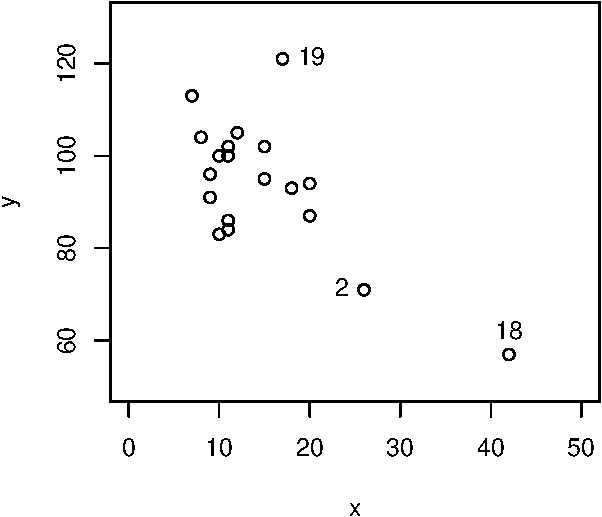
\includegraphics[width=3.25in]{figuras/chap03_sec331_scatter.pdf}
\\ Fonte: Elaborada pelo autor.
\end{center}
\end{figure}

\begin{figure}[H]
\begin{center}
\caption{Boxplot dos resíduos do modelo de regressão normal nos dados originais}
\label{fig:chap03_sec331_boxplot}
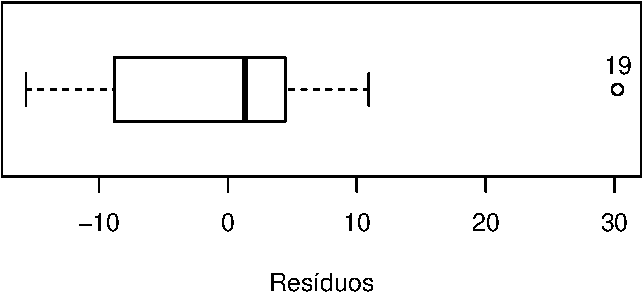
\includegraphics[width=3.5in]{figuras/chap03_sec331_boxplot-crop.pdf}
\\ Fonte: Elaborada pelo autor.
\end{center}
\end{figure}

\begin{figure}[H]
\begin{center}
\caption{$-\log(CPO)$ dos modelos nos dados originais}
\label{fig:chap03_sec331_cpo}
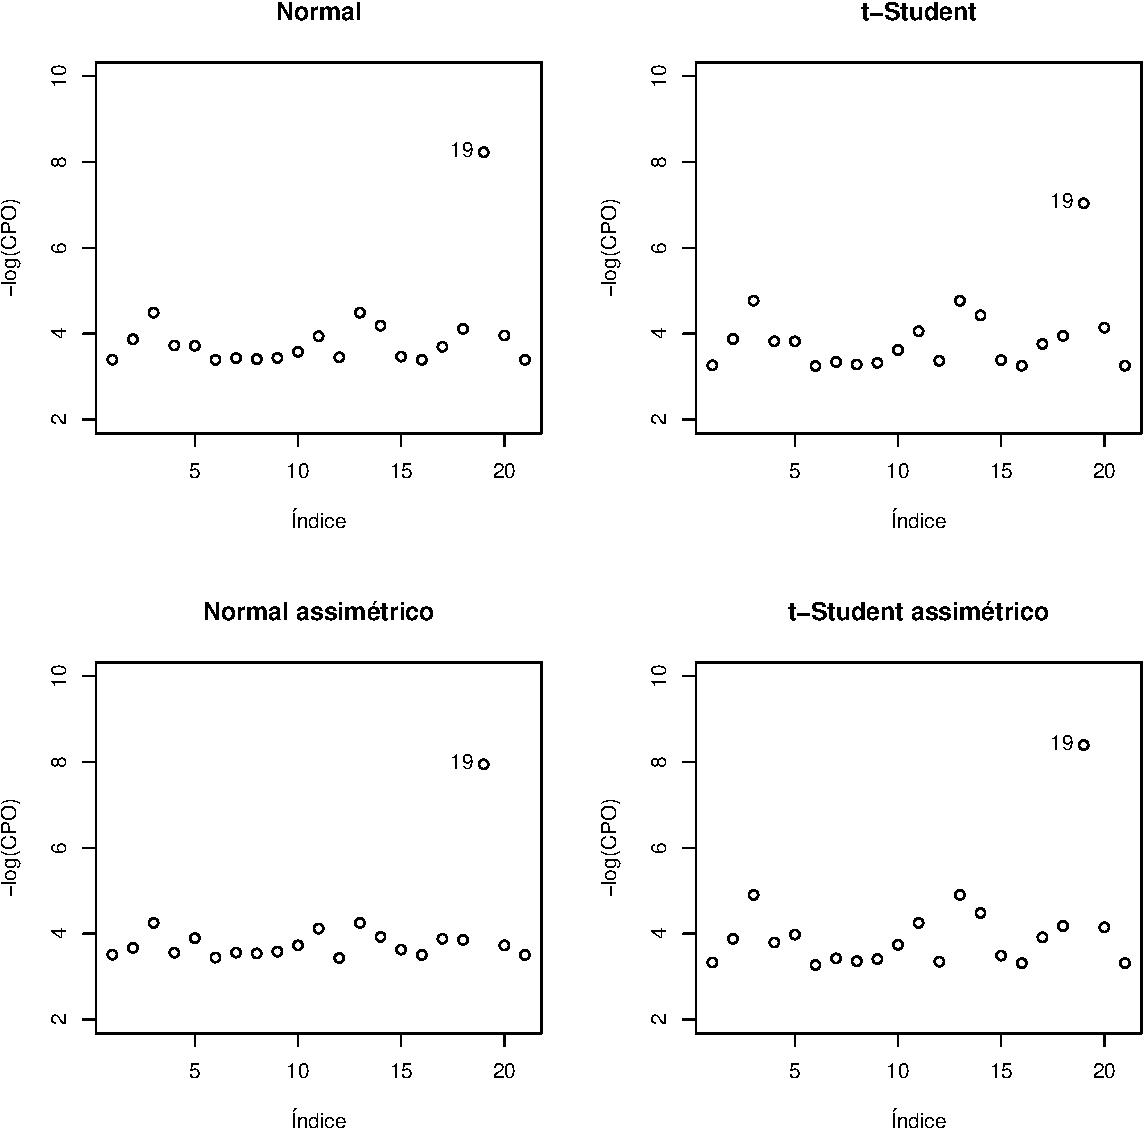
\includegraphics[width=\textwidth]{figuras/chap03_sec331_cpo.pdf}
\\ Fonte: Elaborada pelo autor.
\end{center}
\end{figure}

\begin{figure}[H]
\begin{center}
\caption{Influência global via norma $L_1$ dos modelos nos dados originais}
\label{fig:chap03_sec331_global_l1}
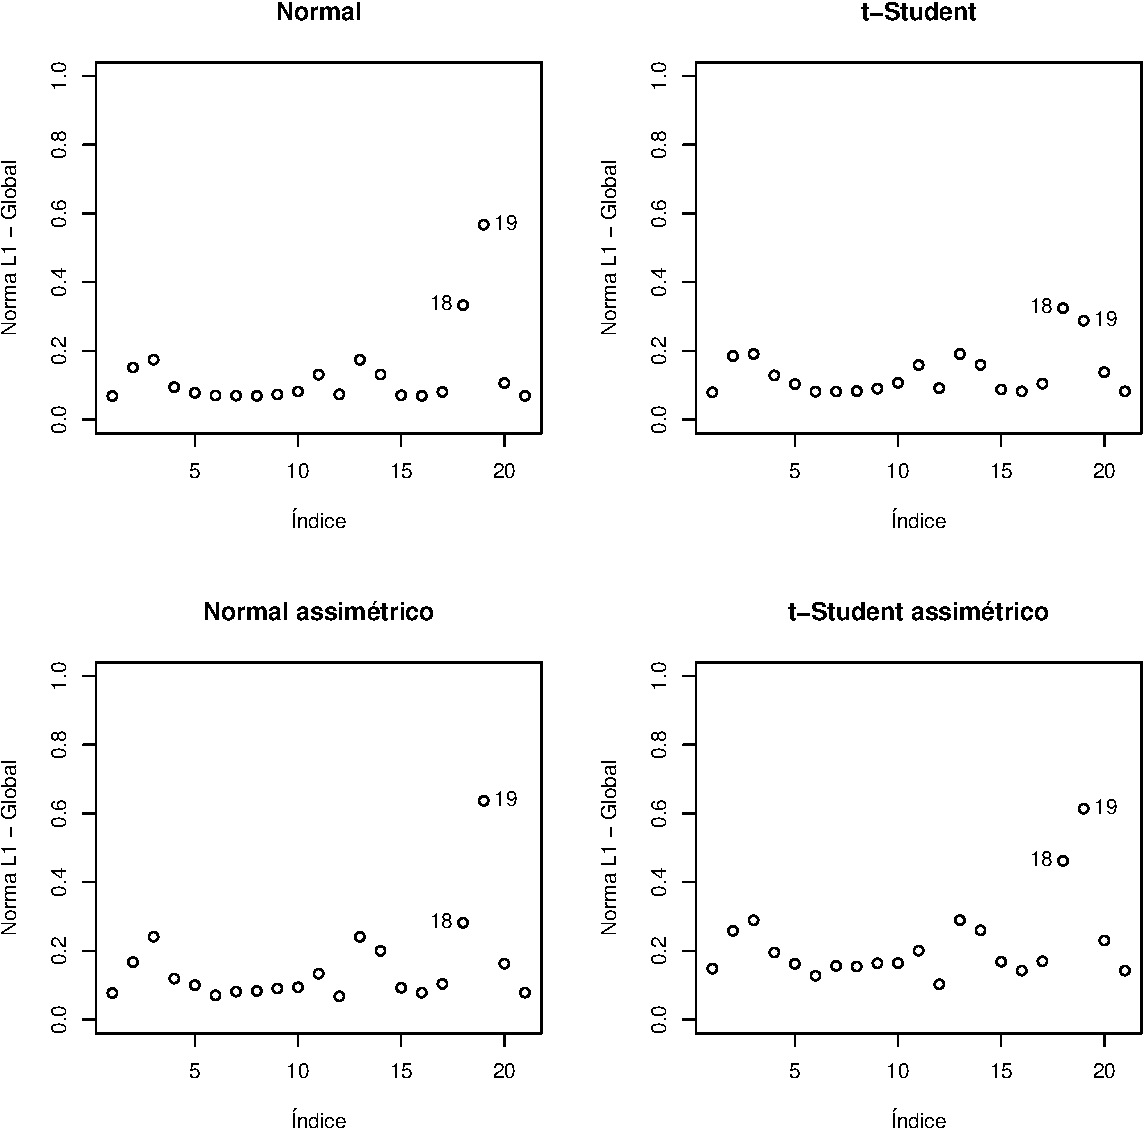
\includegraphics[width=\textwidth]{figuras/chap03_sec331_global_l1.pdf}
\\ Fonte: Elaborada pelo autor.
\end{center}
\end{figure}

\begin{figure}[H]
\begin{center}
\caption{Influência global via divergência de Kullback-Leibler dos modelos nos dados originais}
\label{fig:chap03_sec331_global_kl}
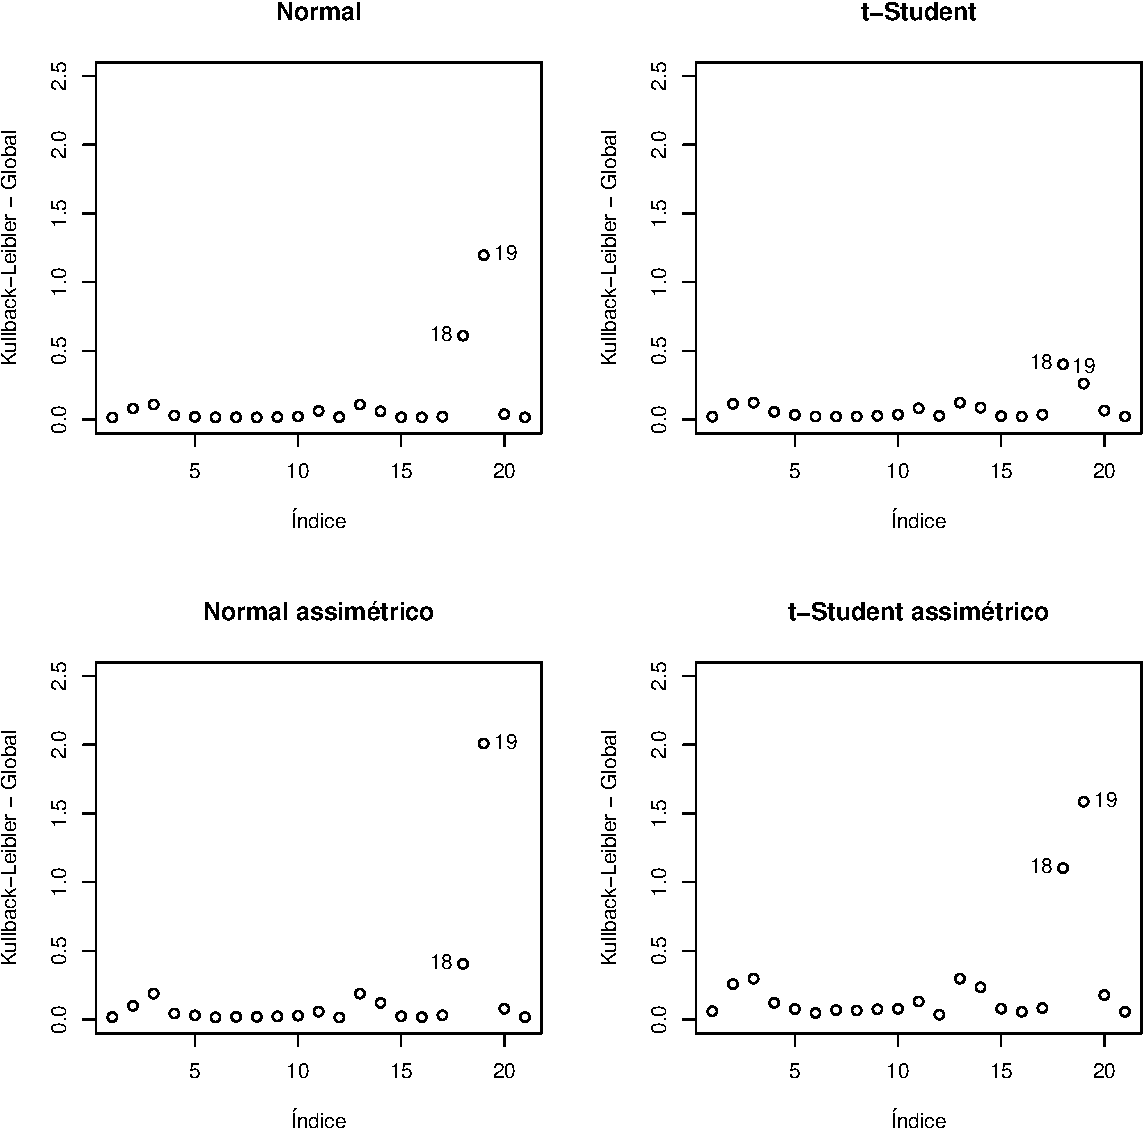
\includegraphics[width=\textwidth]{figuras/chap03_sec331_global_kl.pdf}
\\ Fonte: Elaborada pelo autor.
\end{center}
\end{figure}

\begin{figure}[H]
\begin{center}
\caption{Influência marginal em $\betabf$ via norma $L_1$ dos modelos nos dados originais}
\label{fig:chap03_sec331_marg_l1}
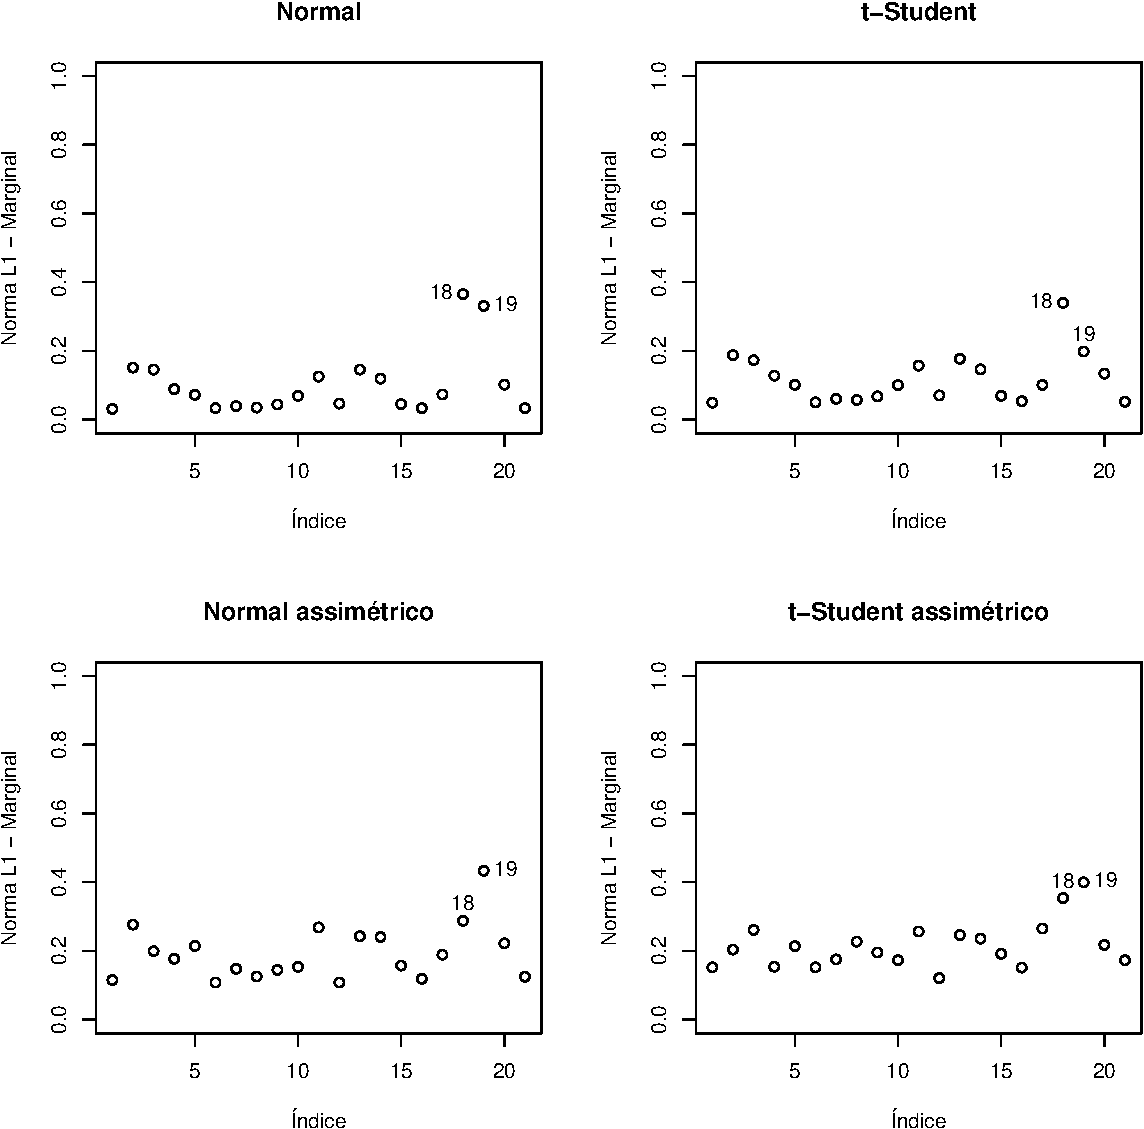
\includegraphics[width=\textwidth]{figuras/chap03_sec331_marg_l1.pdf}
\\ Fonte: Elaborada pelo autor.
\end{center}
\end{figure}

\begin{figure}[H]
\begin{center}
\caption{Influência marginal em $\betabf$ via divergência de Kullback-Leibler dos modelos nos dados originais}
\label{fig:chap03_sec331_marg_kl}
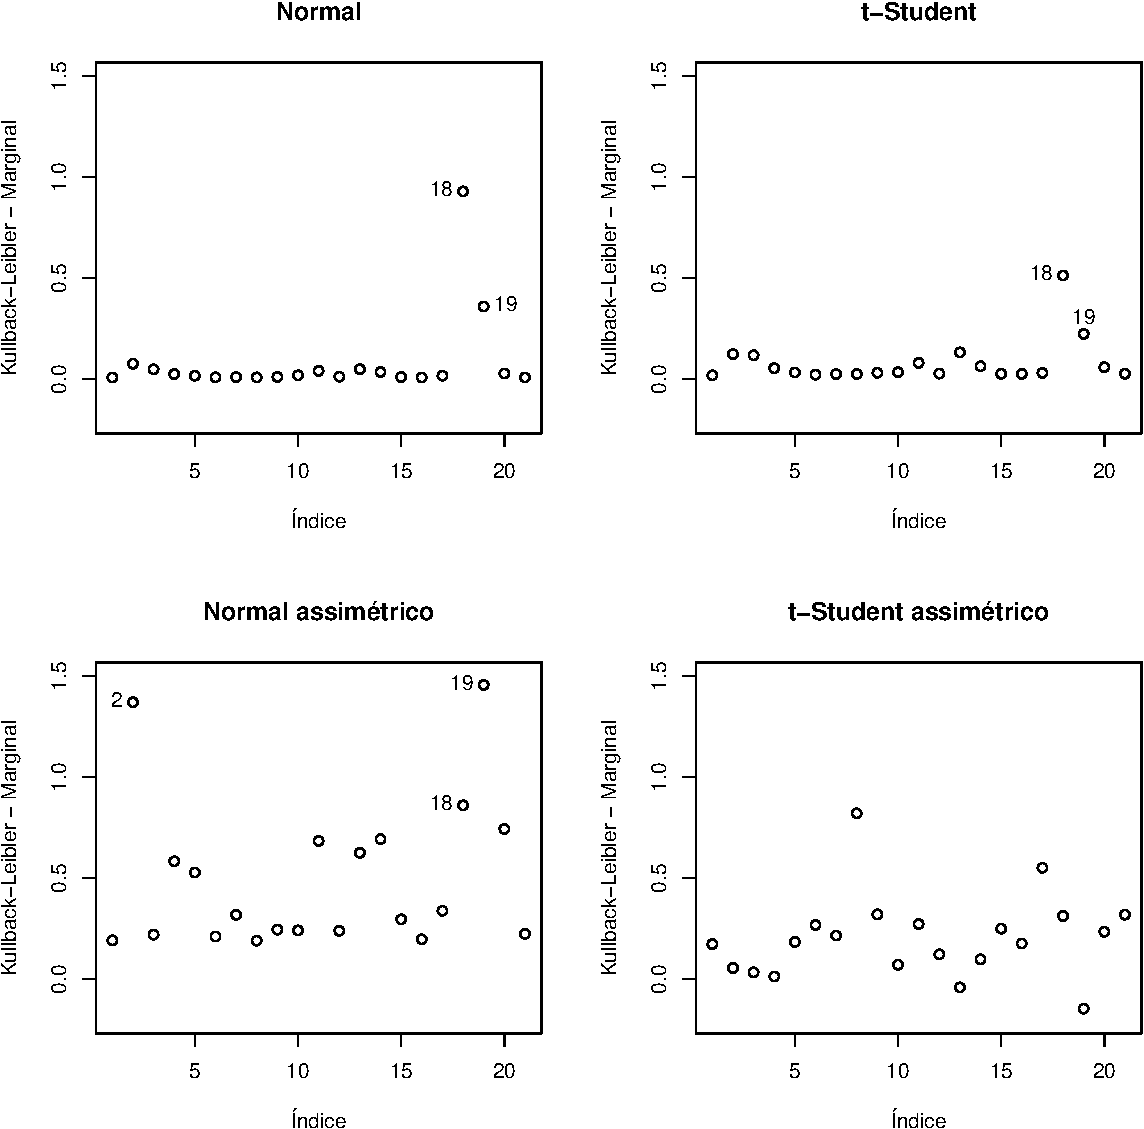
\includegraphics[width=\textwidth]{figuras/chap03_sec331_marg_kl.pdf}
\\ Fonte: Elaborada pelo autor.
\end{center}
\end{figure}

%---------------------------------------------------------------------------------------------%
%---------------------------------------------------------------------------------------------%
%---------------------------------------------------------------------------------------------%
\subsection{Contaminação da observação 19}\label{sec:cont19}

Nesta aplicação, promovemos a contaminação da observação 19 definindo $y_{19} = 60$. Agora podemos observar na Figura \ref{fig:chap03_sec332_boxplot} que o resíduo da distribuição 19 está de acordo com a assimetria negativa da distribuição dos resíduos. Logo, podemos ver na Tabela \ref{tab:chap03_sec332_lpml} que, de fato, os modelos assimétricos possuem um ajuste melhor que os modelos simétricos.

A observação 19 é a mais discrepante em termos do $-\log(CPO)$ em todos os modelos (Figura \ref{fig:chap03_sec332_cpo}). Nas Figuras \ref{fig:chap03_sec332_global_l1} e \ref{fig:chap03_sec332_global_kl} podemos ver que a observação 19 possui uma menor influência global quando comparamos o modelo normal com o modelo $t$-Student e o modelo normal assimétrico com o modelo $t$-assimétrico. Logo, a suposicão de uma cauda mais pesada robustifica os modelos de cauda mais leve. Há um destaque adicional para a observação 11 que, apesar de não ser uma observação discrepante, exerce uma influência nos modelos assimétricos por estar localizado na cauda de menor peso destas distribuições.

Pelas Figuras \ref{fig:chap03_sec332_marg_l1} e \ref{fig:chap03_sec332_marg_kl} notamos que a influência marginal da observação 19 nos modelos simétricos é bem reduzida. Já nos modelos assimétricos, vemos que a influência da observação 19 é maior no modelo normal assimétrico do que no modelo $t$-assimétrico. Logo, há um indício que o modelo $t$-assimétrico é menos influenciado marginalmente do que o modelo normal assimétrico.  

\begin{table}[H]
\begin{center}
\caption{LPML dos modelos contaminando a observação 19}
\label{tab:chap03_sec332_lpml}
\begin{tabular}{cccc}
 Normal & $t$-Student & Normal assimétrica  & $t$-assimétrica \\ \hline
-81.6 & -81.38 & -78.73 & -79.7 \\ \hline
\end{tabular}
\\ Fonte: Elaborada pelo autor.
\end{center}
\end{table}

\begin{figure}[H]
\begin{center}
\caption{Diagrama de dispersão contaminando a observação 19}
\label{fig:chap03_sec332_scatter}
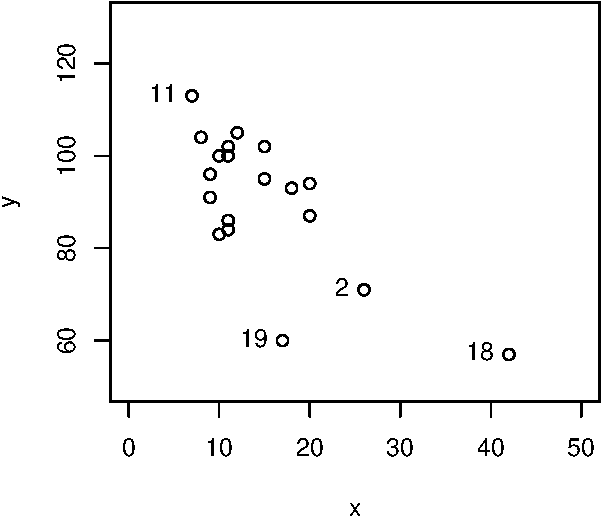
\includegraphics[width=3.25in]{figuras/chap03_sec332_scatter.pdf}
\\ Fonte: Elaborada pelo autor.
\end{center}
\end{figure}

\begin{figure}[H]
\begin{center}
\caption{Boxplot dos resíduos do modelo de regressão normal contaminando a observação 19}
\label{fig:chap03_sec332_boxplot}
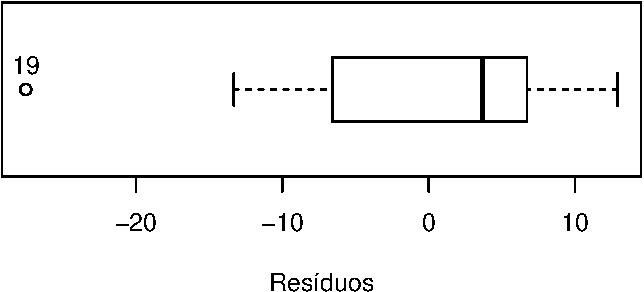
\includegraphics[width=3.5in]{figuras/chap03_sec332_boxplot-crop.pdf}
\\ Fonte: Elaborada pelo autor.
\end{center}
\end{figure}

\begin{figure}[H]
\begin{center}
\caption{$-\log(CPO)$ dos modelos contaminando a observação 19}
\label{fig:chap03_sec332_cpo}
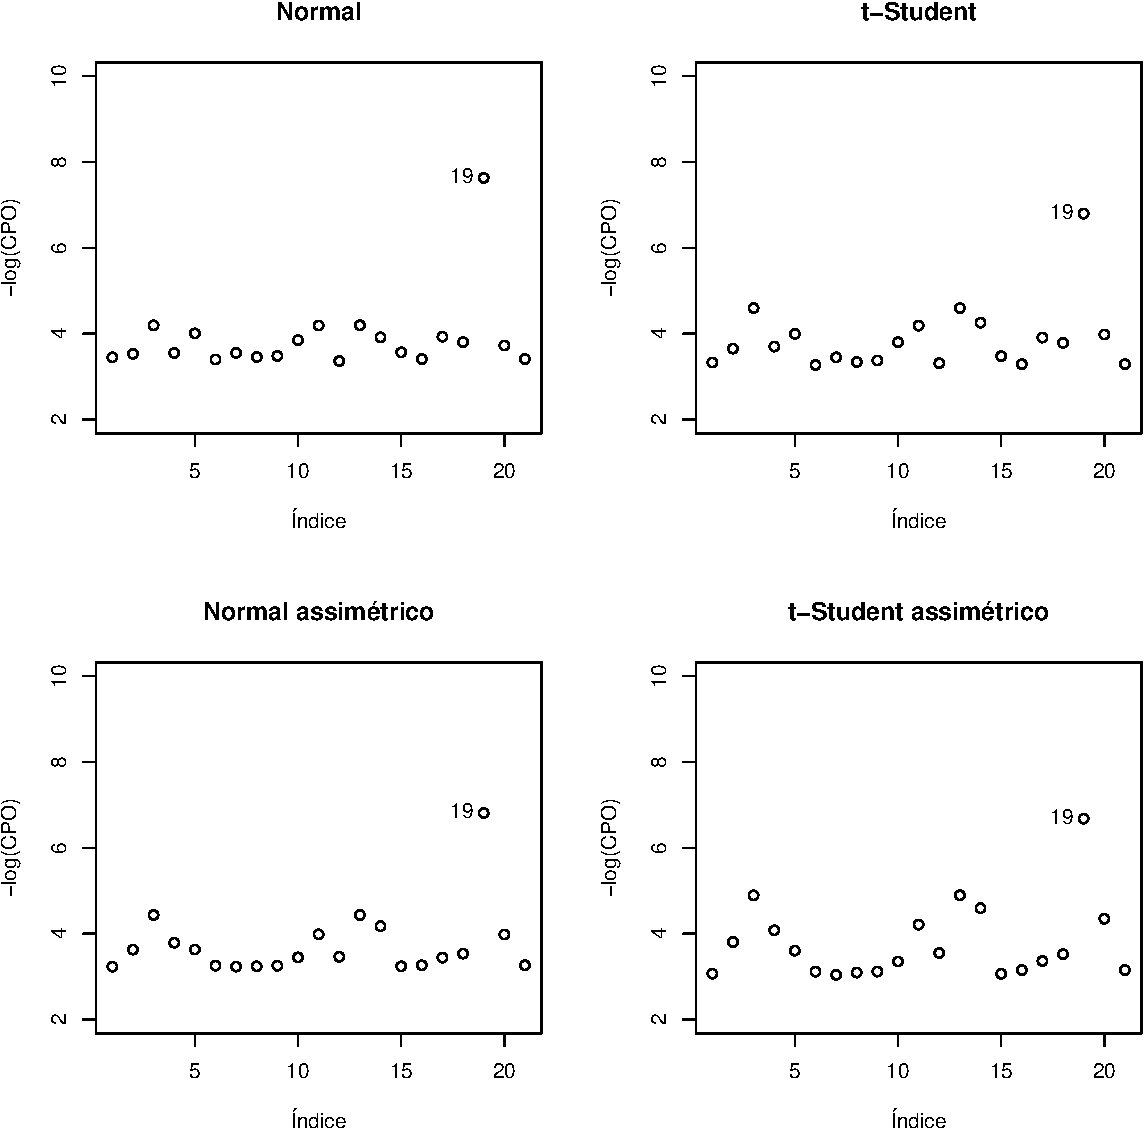
\includegraphics[width=\textwidth]{figuras/chap03_sec332_cpo.pdf}
\\ Fonte: Elaborada pelo autor.
\end{center}
\end{figure}

\begin{figure}[H]
\begin{center}
\caption{Influência global via norma $L_1$ dos modelos contaminando a observação 19}
\label{fig:chap03_sec332_global_l1}
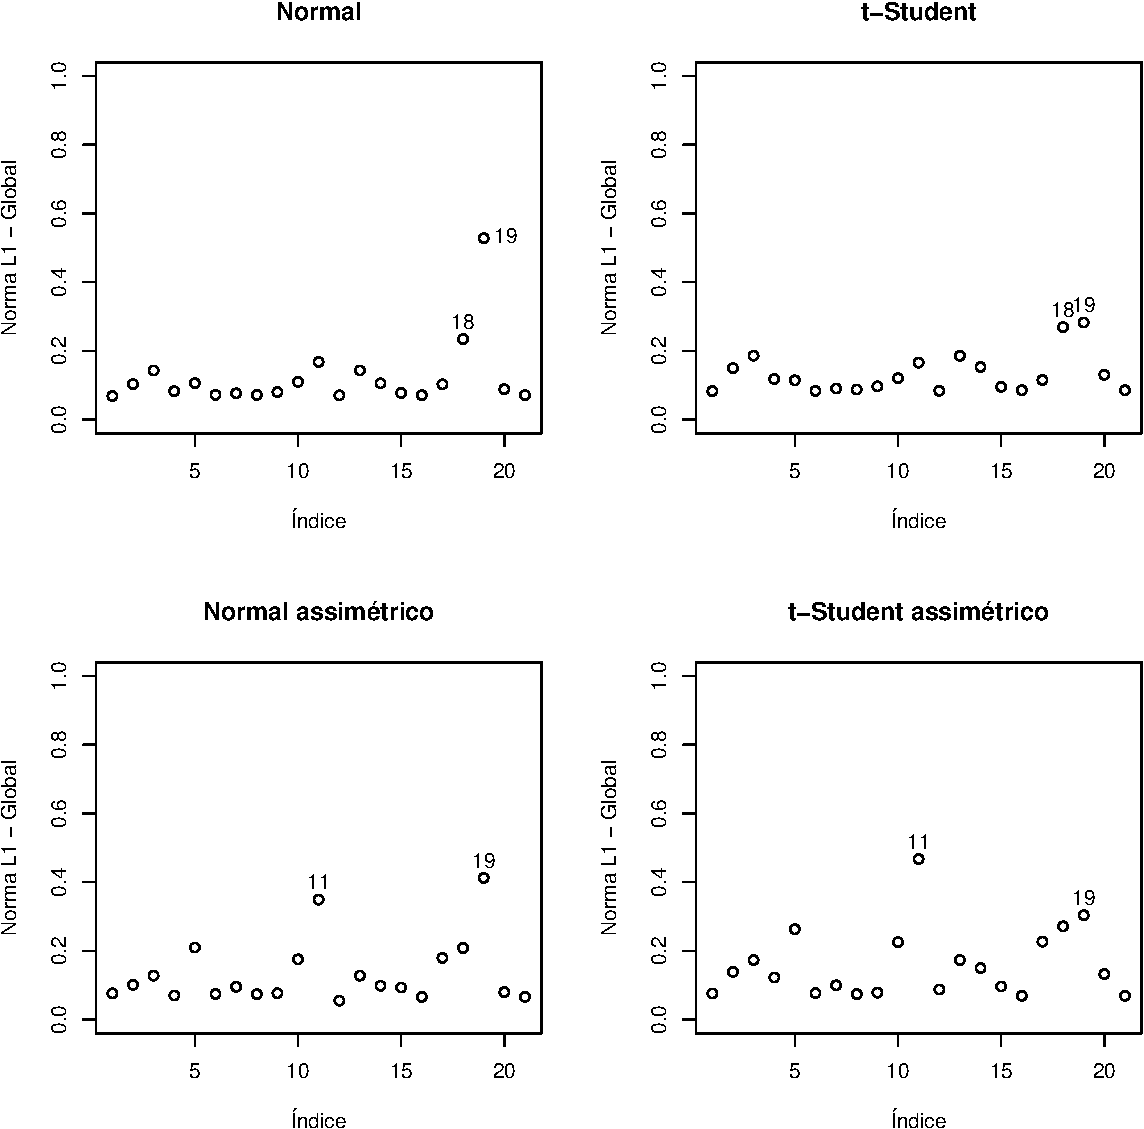
\includegraphics[width=\textwidth]{figuras/chap03_sec332_global_l1.pdf}
\\ Fonte: Elaborada pelo autor.
\end{center}
\end{figure}

\begin{figure}[H]
\begin{center}
\caption{Influência global via divergência de Kullback-Leibler dos modelos contaminando a observação 19}
\label{fig:chap03_sec332_global_kl}
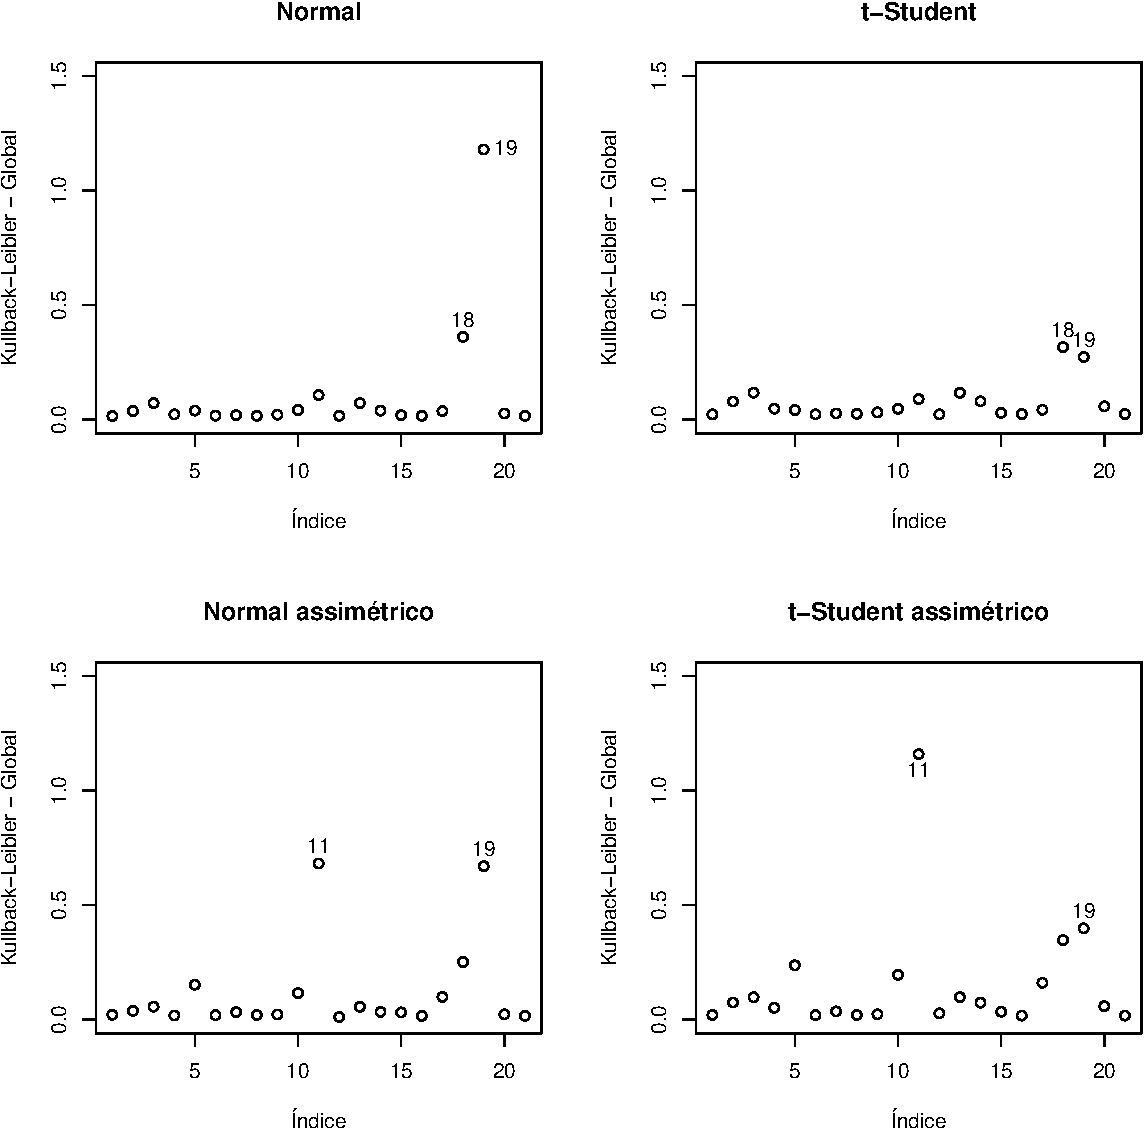
\includegraphics[width=\textwidth]{figuras/chap03_sec332_global_kl.pdf}
\\ Fonte: Elaborada pelo autor.
\end{center}
\end{figure}

\begin{figure}[H]
\begin{center}
\caption{Influência marginal em $\betabf$ via norma $L_1$ dos modelos contaminando a observação 19}
\label{fig:chap03_sec332_marg_l1}
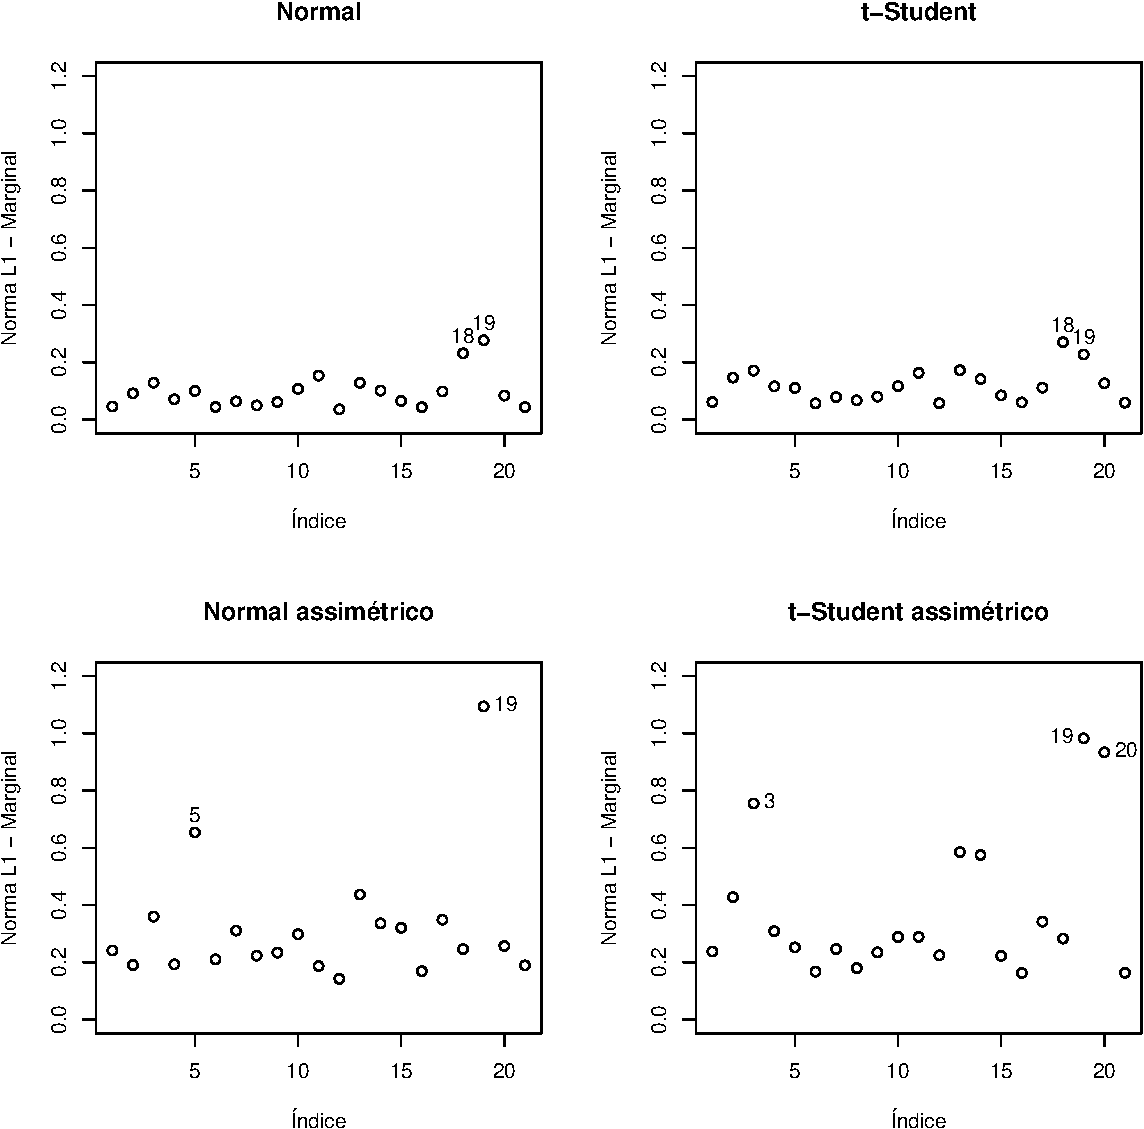
\includegraphics[width=\textwidth]{figuras/chap03_sec332_marg_l1.pdf}
\\ Fonte: Elaborada pelo autor.
\end{center}
\end{figure}

\begin{figure}[H]
\begin{center}
\caption{Influência marginal em $\betabf$ via divergência de Kullback-Leibler dos modelos contaminando a observação 19}
\label{fig:chap03_sec332_marg_kl}
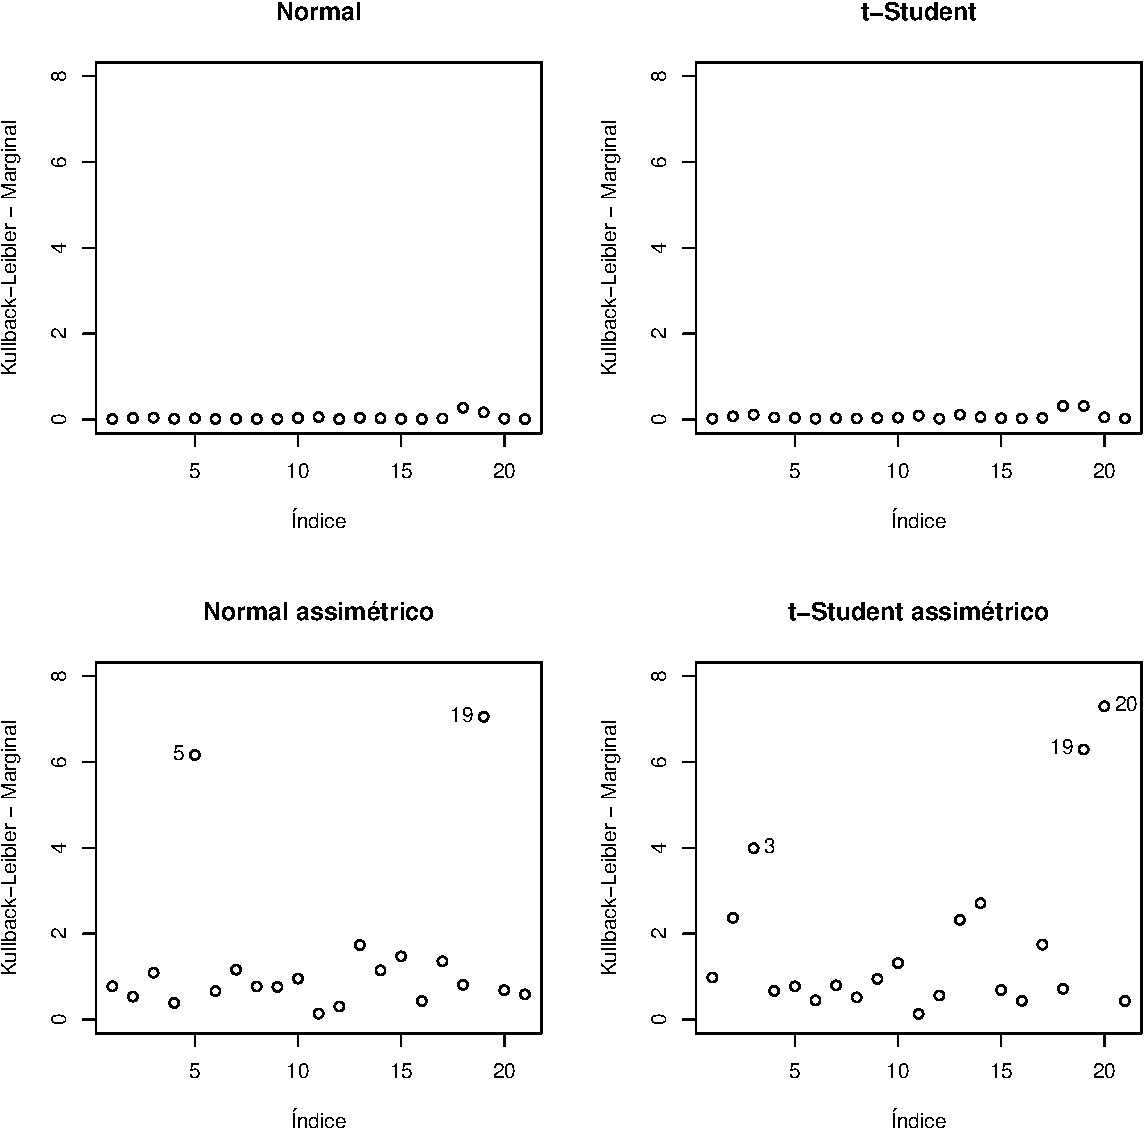
\includegraphics[width=\textwidth]{figuras/chap03_sec332_marg_kl.pdf}
\\ Fonte: Elaborada pelo autor.
\end{center}
\end{figure}

%---------------------------------------------------------------------------------------------%
%---------------------------------------------------------------------------------------------%
%---------------------------------------------------------------------------------------------%
\subsection{Contaminação da observação 14}

Nesta aplicação contaminamos a observação 14 fazendo $y_{14} = 60$. Com esta contaminação, podemos observar as observações 14 e 19 com resíduo alto (Figura \ref{fig:chap03_sec333_boxplot}). A existência de resíduos altos em ambos lados da distribuição justifica o melhor ajustes dos modelos simétricos frente aos modelos assimétricos (Tabela \ref{tab:chap03_sec333_lpml}).

Vemos na Figura \ref{fig:chap03_sec333_cpo} que em quase todos os modelos a observação 14 é um pouco mais discrepante que a 19. Porém, no modelo $t$-assimétrico, a observação 19 é mais discrepante que a 14 por estar localizada na cauda mais leve desta distribuição. Podemos ver nas Figuras \ref{fig:chap03_sec333_global_l1} e \ref{fig:chap03_sec333_global_kl} que o modelo $t$-Student é aquele em que as observações 14, 18 e 19 são menos influentes de forma global. Por outro lado, a observação 19 exerce uma grande influência no modelo $t$-assimétrico.

Analisando a influência marginal vemos na Figura \ref{fig:chap03_sec333_marg_l1} que a observação 19 exerce uma influência menor nos modelos simétricos do que nos modelos assimétricos. Isto pode acontecer por ela estar localizada na cauda de menor peso destas distribuições assimétricas.

\begin{table}[H]
\begin{center}
\caption{LPML dos modelos contaminando a observação 14}
\label{tab:chap03_sec333_lpml}
\begin{tabular}{cccc}
 Normal & $t$-Student & Normal assimétrica  & $t$-assimétrica \\ \hline
-87.49 & -85.31 & -87.8 & -90.68 \\ \hline
\end{tabular}
\\
Fonte: Elaborada pelo autor.
\end{center}
\end{table}


\begin{figure}[H]
\begin{center}
\caption{Diagrama de dispersão contaminando a observação 14}
\label{fig:chap03_sec333_scatter}
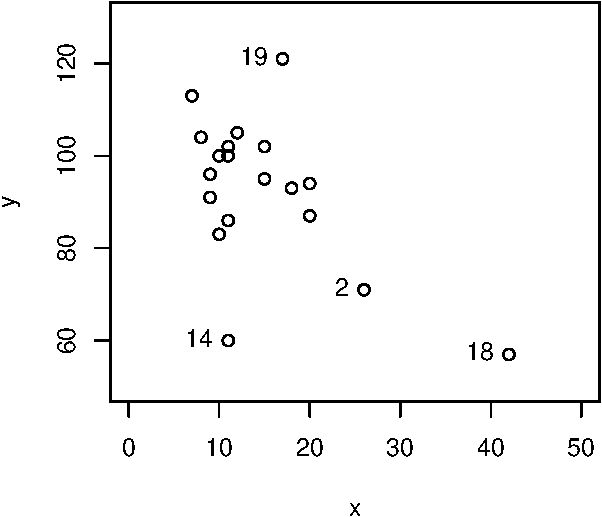
\includegraphics[width=3.25in]{figuras/chap03_sec333_scatter.pdf}
\\ Fonte: Elaborada pelo autor.
\end{center}
\end{figure}

\begin{figure}[H]
\begin{center}
\caption{Boxplot dos resíduos do modelo de regressão normal contaminando a observação 14}
\label{fig:chap03_sec333_boxplot}
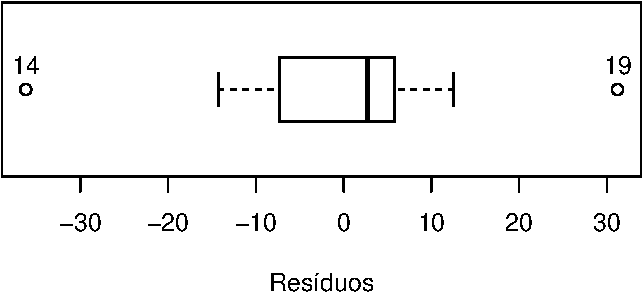
\includegraphics[width=3.5in]{figuras/chap03_sec333_boxplot-crop.pdf}
\\ Fonte: Elaborada pelo autor.
\end{center}
\end{figure}

\begin{figure}[H]
\begin{center}
\caption{$-\log(CPO)$ dos modelos contaminando a observação 14}
\label{fig:chap03_sec333_cpo}
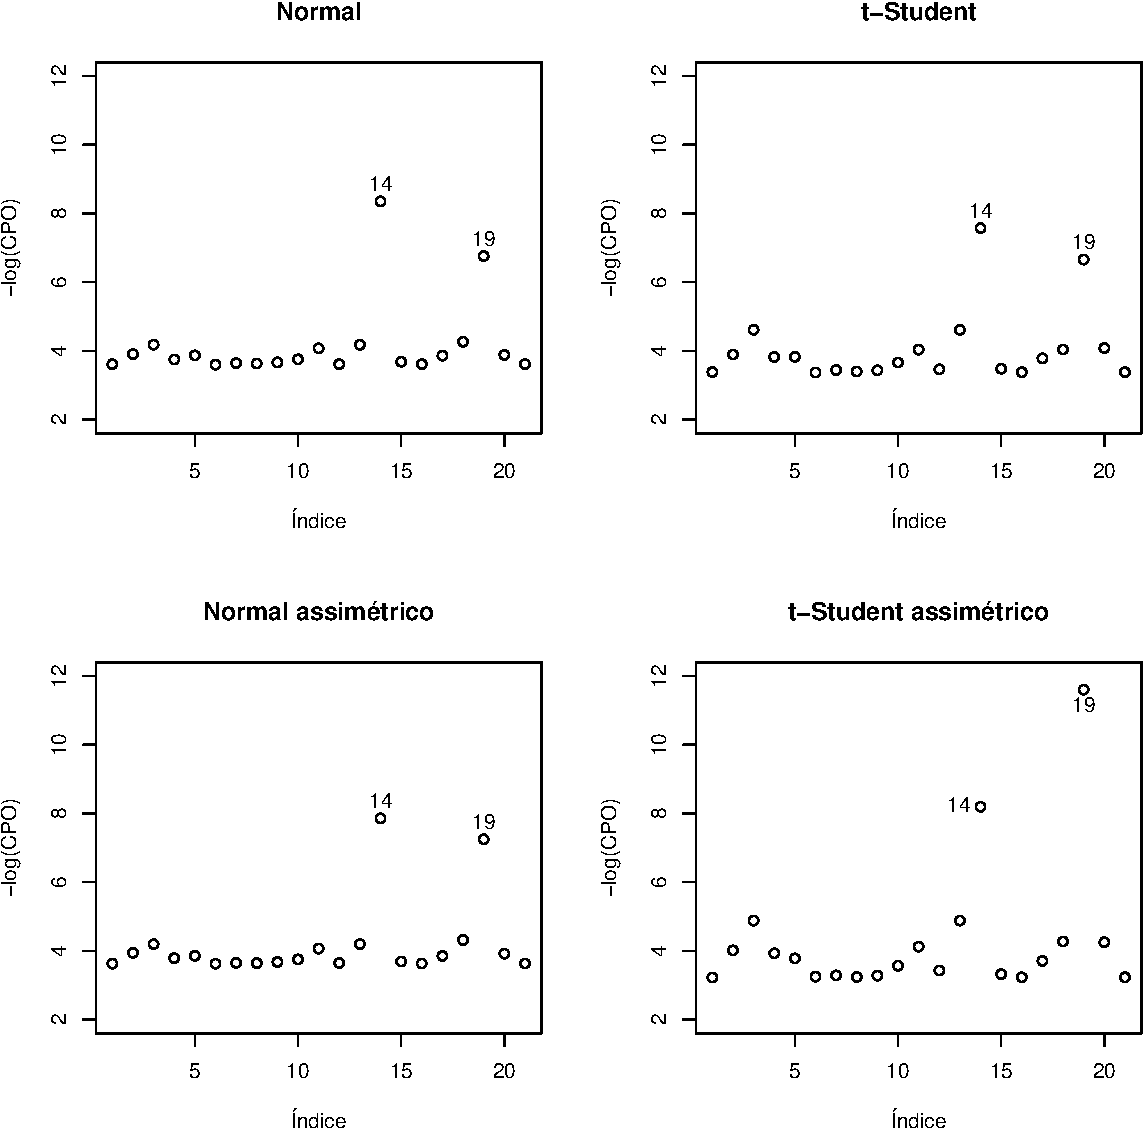
\includegraphics[width=\textwidth]{figuras/chap03_sec333_cpo.pdf}
\\ Fonte: Elaborada pelo autor.
\end{center}
\end{figure}

\begin{figure}[H]
\begin{center}
\caption{Influência global via norma $L_1$ dos modelos contaminando a observação 14}
\label{fig:chap03_sec333_global_l1}
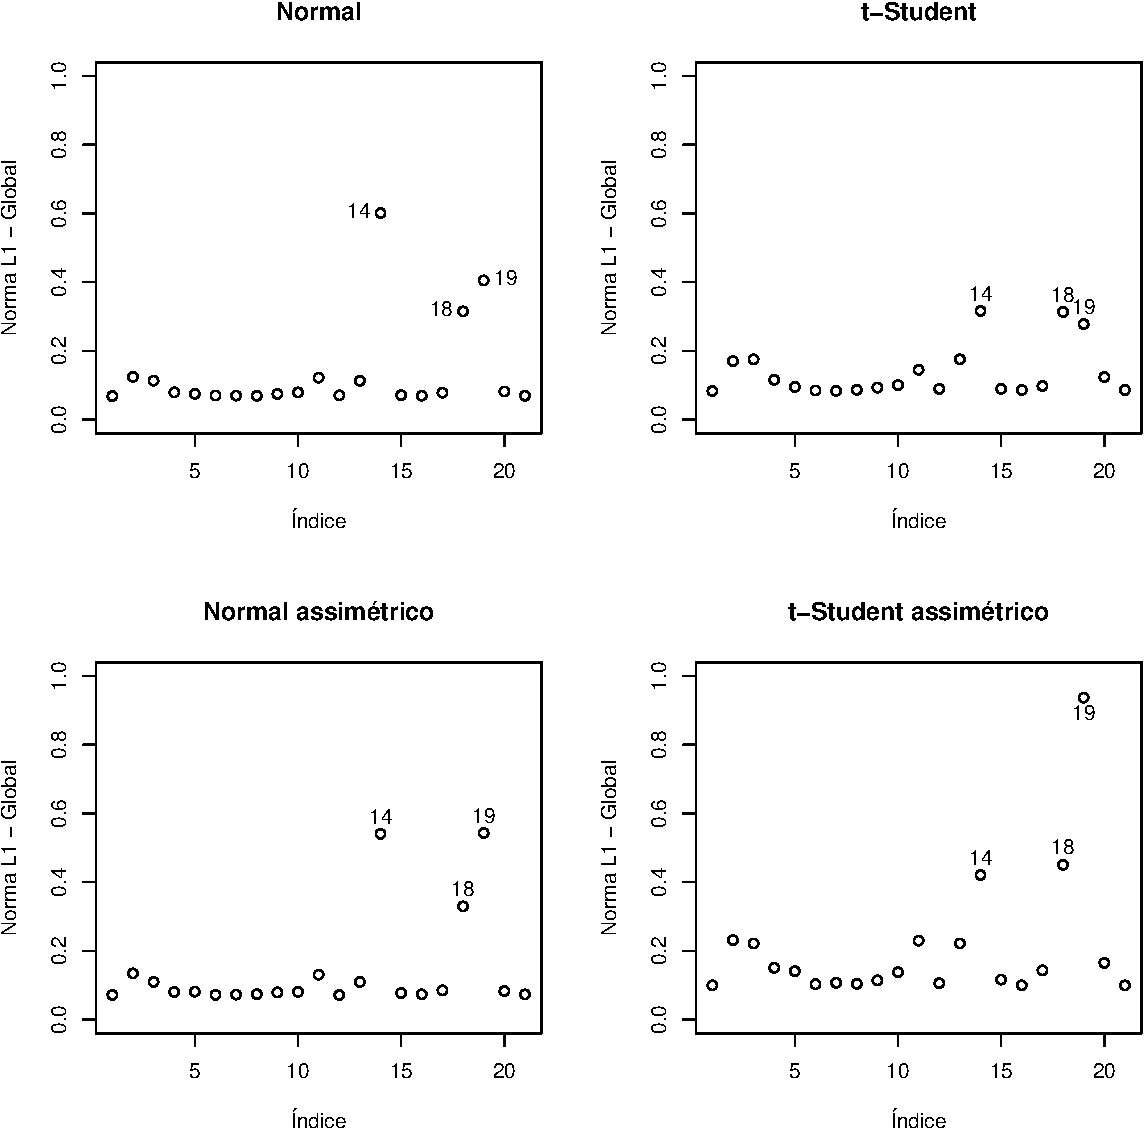
\includegraphics[width=\textwidth]{figuras/chap03_sec333_global_l1.pdf}
\\ Fonte: Elaborada pelo autor.
\end{center}
\end{figure}

\newpage
\begin{figure}[!h]
\begin{center}
\caption{Influência global via divergência de Kullback-Leibler dos modelos contaminando a observação 14}
\label{fig:chap03_sec333_global_kl}
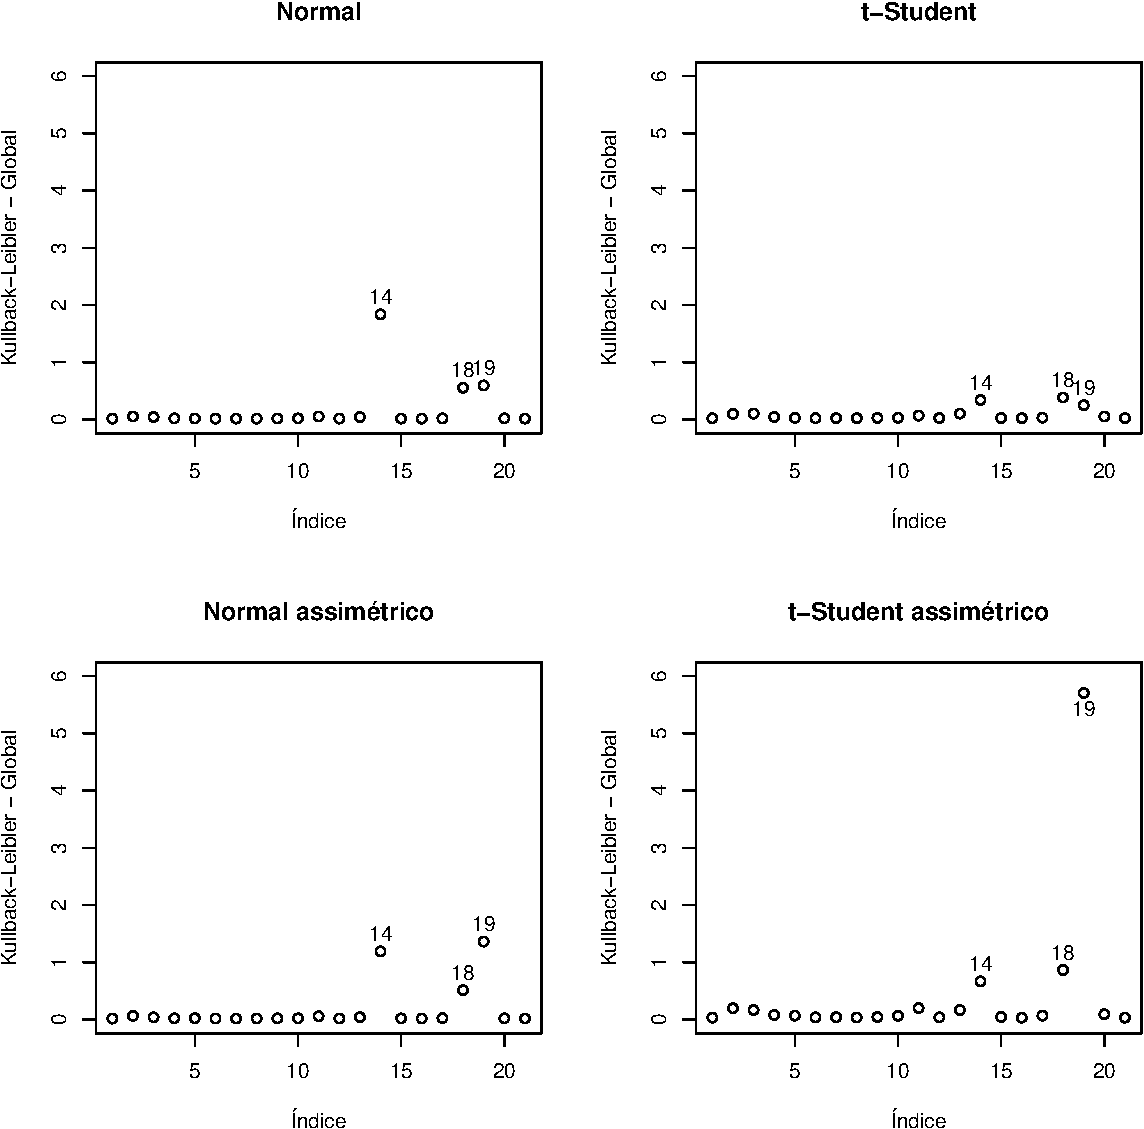
\includegraphics[width=\textwidth]{figuras/chap03_sec333_global_kl.pdf}
\\ Fonte: Elaborada pelo autor.
\end{center}
\end{figure}

\newpage
\begin{figure}[!h]
\begin{center}
\caption{Influência marginal em $\betabf$ via norma $L_1$ dos modelos contaminando a observação 14}
\label{fig:chap03_sec333_marg_l1}
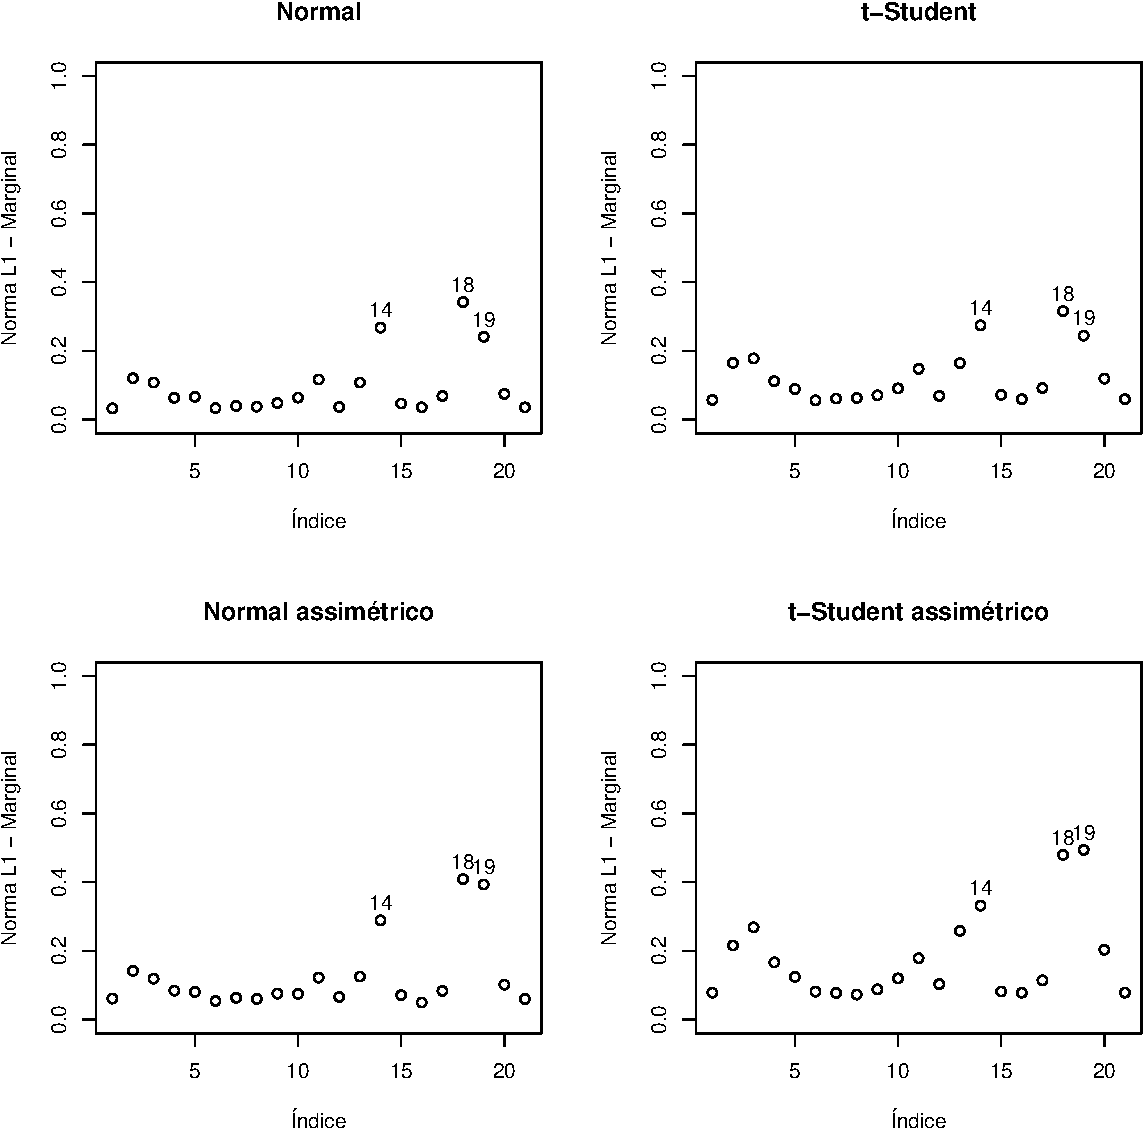
\includegraphics[width=\textwidth]{figuras/chap03_sec333_marg_l1.pdf}
\\ Fonte: Elaborada pelo autor.
\end{center}
\end{figure}

\begin{figure}[H]
\begin{center}
\caption{Influência marginal em $\betabf$ via divergência de Kullback-Leibler dos modelos contaminando a observação 14}
\label{fig:chap03_sec333_marg_kl}
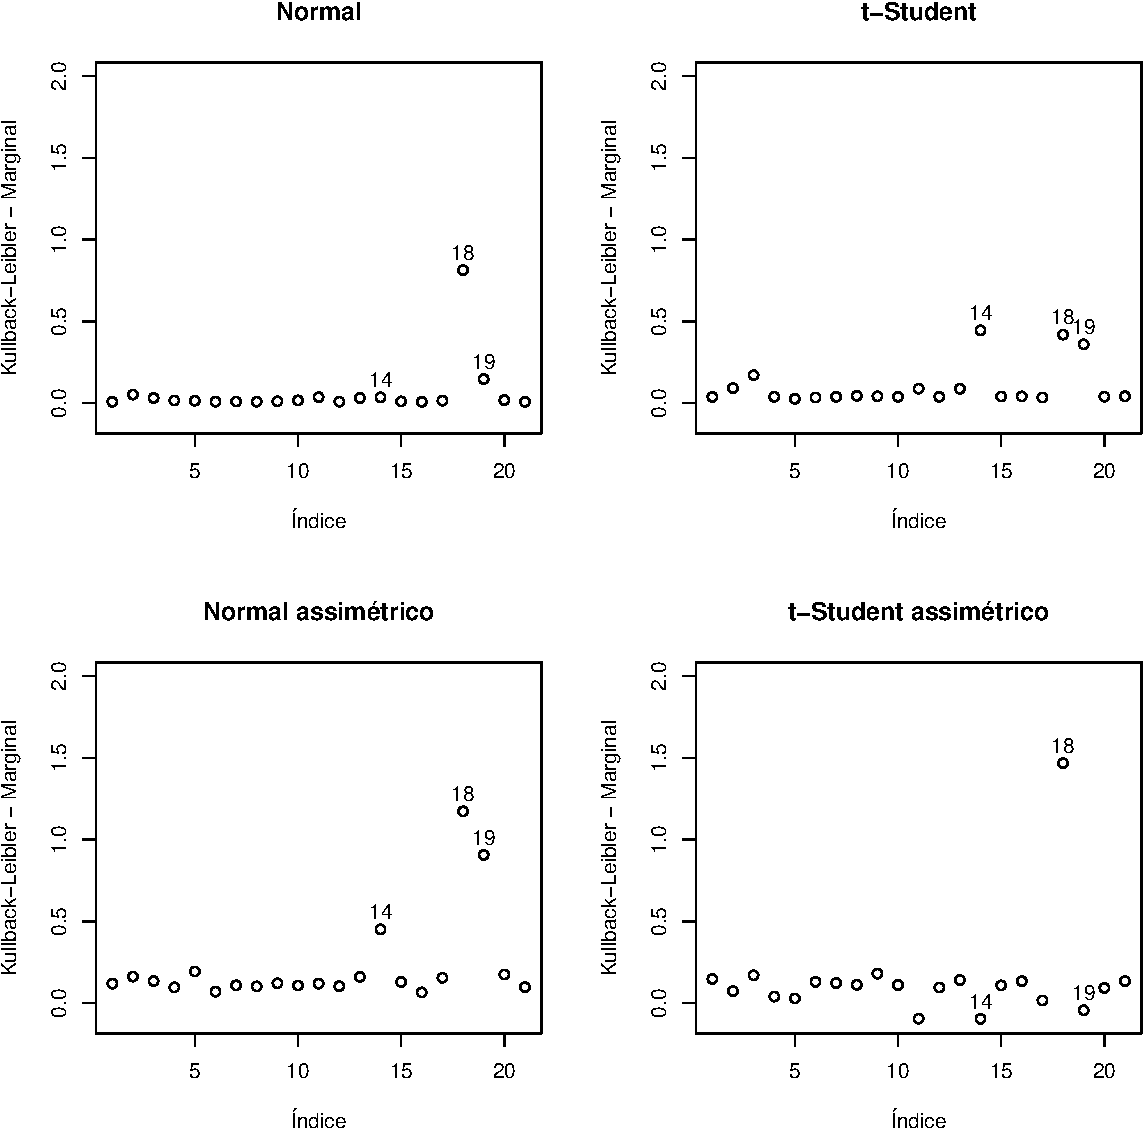
\includegraphics[width=\textwidth]{figuras/chap03_sec333_marg_kl.pdf}
\\ Fonte: Elaborada pelo autor.
\end{center}
\end{figure}
%---------------------------------------------------------------------------------------------%
%---------------------------------------------------------------------------------------------%
%---------------------------------------------------------------------------------------------%
\subsection{Contaminação das observações 14 e 19}

Nesta última aplicação promovemos a contaminação das observações 14 e 19 simultaneamente, fazendo $y_{14}=y_{19}=60$. Assim, agora, as duas observações de maior resíduo estão na direção da assimetria da distribuição dos resíduos (Figura \ref{fig:chap03_sec334_boxplot}). Neste caso, os modelos assimétricos mostram um ajuste muito superior aos simétricos (Tabela \ref{fig:chap03_sec334_lpml}).

As observações 14 e 19 são discrepantes em todos os modelos propostos (Figura \ref{fig:chap03_sec334_cpo}) sendo a observação 14, de maior resíduo, a mais discrepante. Vemos nas Figuras \ref{fig:chap03_sec334_global_l1} e \ref{fig:chap03_sec334_global_kl} que os modelos $t$-Student e $t$-assimétrico são aqueles menos influenciados de forma global pela observação 14.

Apesar de apresentarem influência global, as observações 14 e 19 possuem uma baixa influência marginal nos modelos simétricos. Já sob os modelos assimétricos, a observação 14 aparenta exercer uma maior influência sob o modelo $t$-assimétrico do que sob o modelo normal assimétrico. Contudo, como os valores obtidos tanto para norma $L_1$ quanto para a divergência Kullback-Leibler aparentam uma maior instabilidade nos modelos assimétricos do que nos modelos simétricos (a norma $L_1$ excede o domínio $[0,1]$, por exemplo), devemos ter cuidado ao considerar estes resultados.

\begin{table}[!h]
\begin{center}
\caption{LPML dos modelos contaminando as observações 14 e 19}
\label{fig:chap03_sec334_lpml}
\begin{tabular}{cccc}
 Normal & $t$-Student & Normal assimétrica  & $t$-assimétrica \\ \hline
-86.15 & -84.95 & -80.92 & -81.58 \\ \hline
\end{tabular}
\\
Fonte: Elaborada pelo autor.
\end{center}
\end{table}


\begin{figure}[H]
\begin{center}
\caption{Diagrama de dispersão contaminando as observações 14 e 19}
\label{fig:chap03_sec334_scatter}
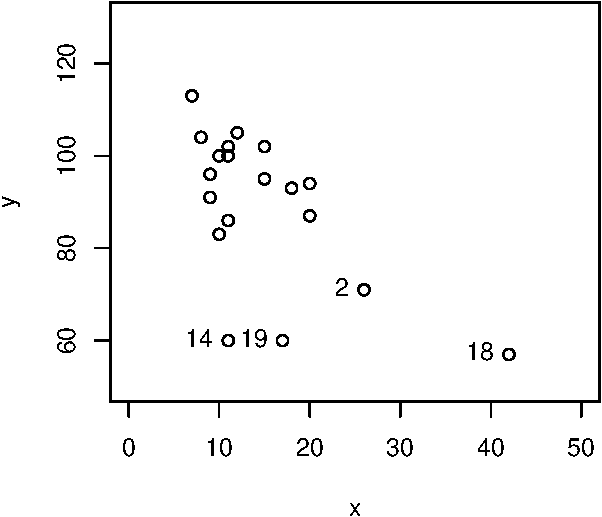
\includegraphics[width=3.25in]{figuras/chap03_sec334_scatter.pdf}
\\ Fonte: Elaborada pelo autor.
\end{center}
\end{figure}

\begin{figure}[H]
\begin{center}
\caption{Boxplot dos resíduos do modelo de regressão normal contaminando as observações 14 e 19}
\label{fig:chap03_sec334_boxplot}
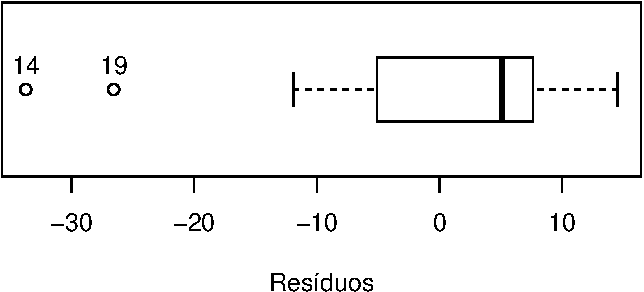
\includegraphics[width=3.5in]{figuras/chap03_sec334_boxplot-crop.pdf}
\\ Fonte: Elaborada pelo autor.
\end{center}
\end{figure}

\begin{figure}[H]
\begin{center}
\caption{$-\log(CPO)$ dos modelos contaminando as observações 14 e 19}
\label{fig:chap03_sec334_cpo}
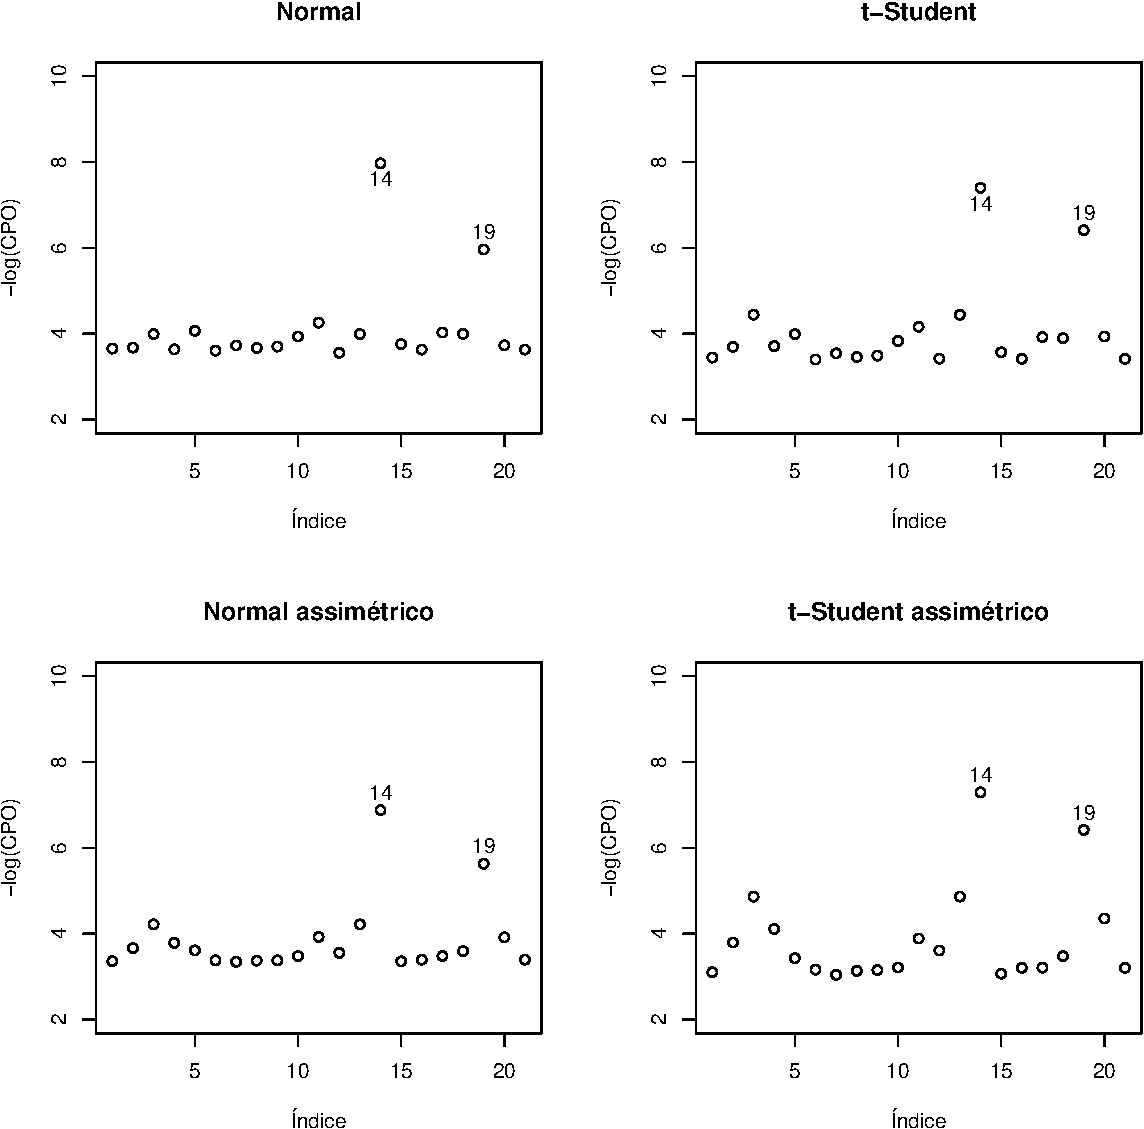
\includegraphics[width=\textwidth]{figuras/chap03_sec334_cpo.pdf}
\\ Fonte: Elaborada pelo autor.
\end{center}
\end{figure}

\begin{figure}[H]
\begin{center}
\caption{Influência global via norma $L_1$ dos modelos contaminando as observações 14 e 19}
\label{fig:chap03_sec334_global_l1}
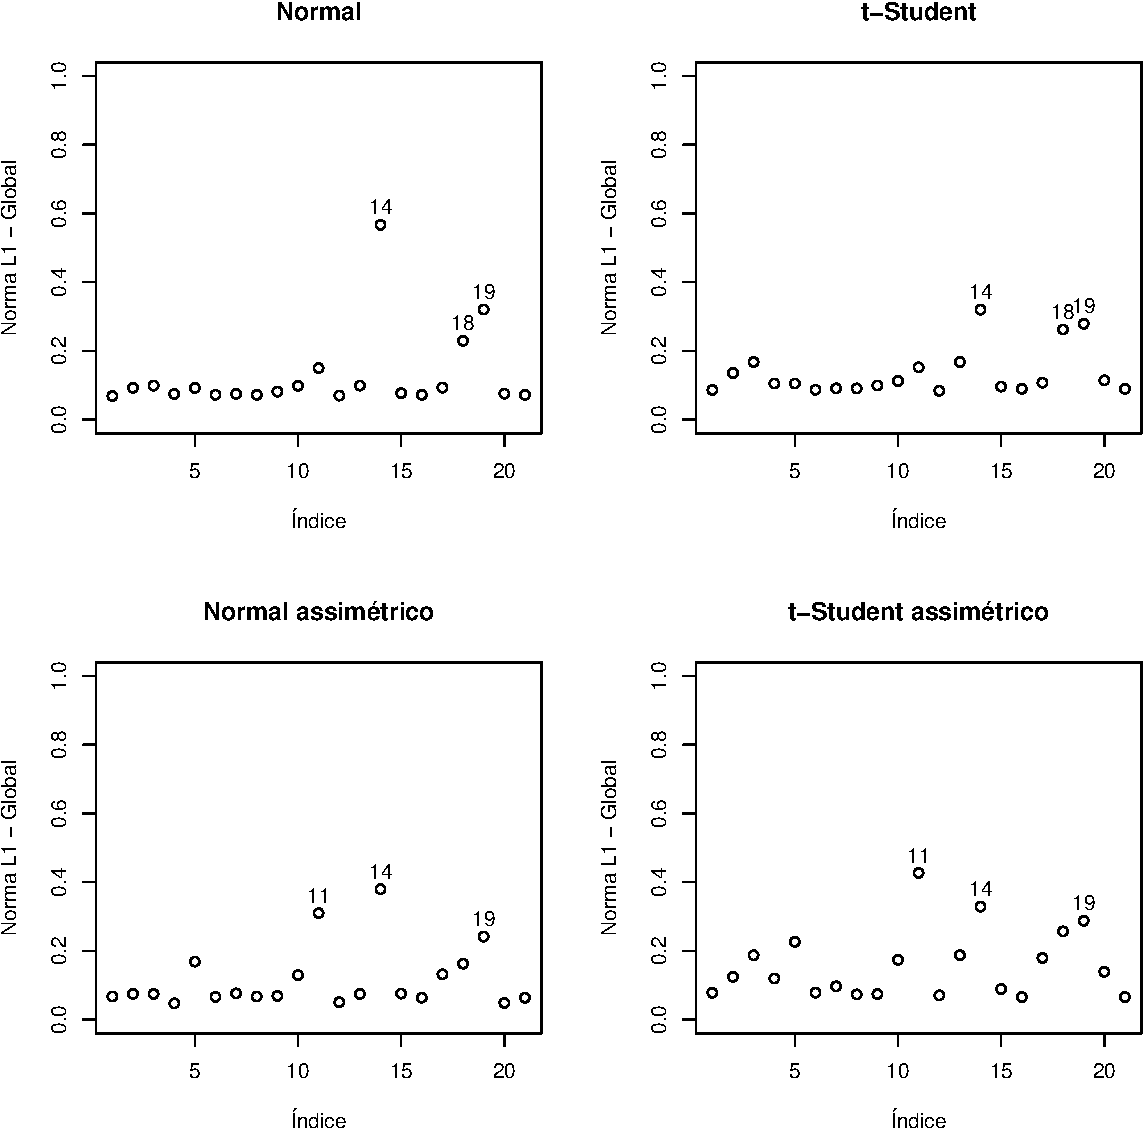
\includegraphics[width=\textwidth]{figuras/chap03_sec334_global_l1.pdf}
\\ Fonte: Elaborada pelo autor.
\end{center}
\end{figure}

\begin{figure}[H]
\begin{center}
\caption{Influência global via divergência de Kullback-Leibler dos modelos contaminando as observações 14 e 19}
\label{fig:chap03_sec334_global_kl}
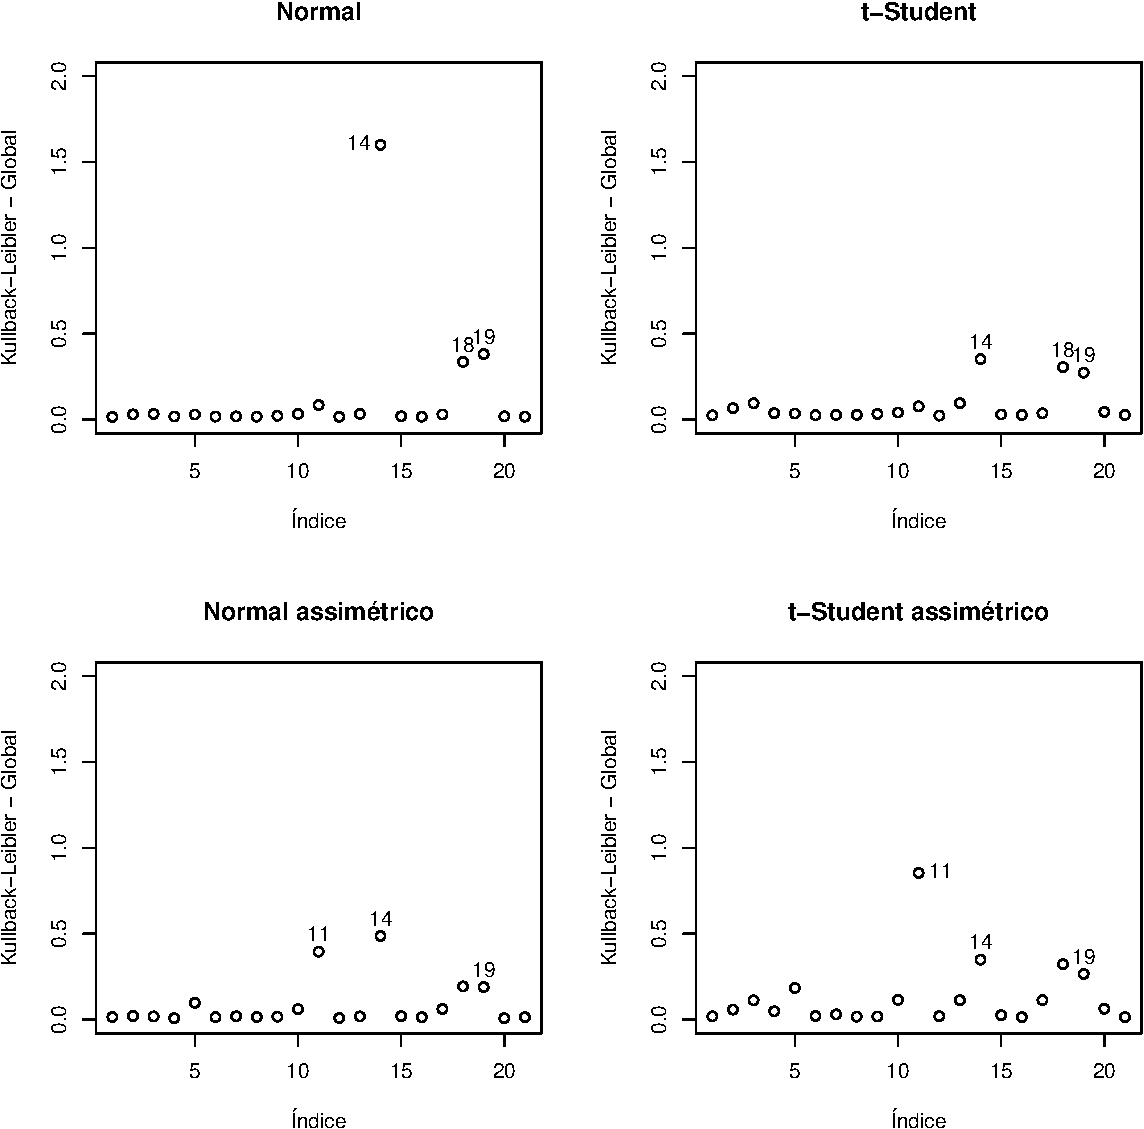
\includegraphics[width=\textwidth]{figuras/chap03_sec334_global_kl.pdf}
\\ Fonte: Elaborada pelo autor.
\end{center}
\end{figure}

\begin{figure}[H]
\begin{center}
\caption{Influência marginal em $\betabf$ via norma $L_1$ dos modelos contaminando as observações 14 e 19}
\label{fig:chap03_sec334_marg_l1}
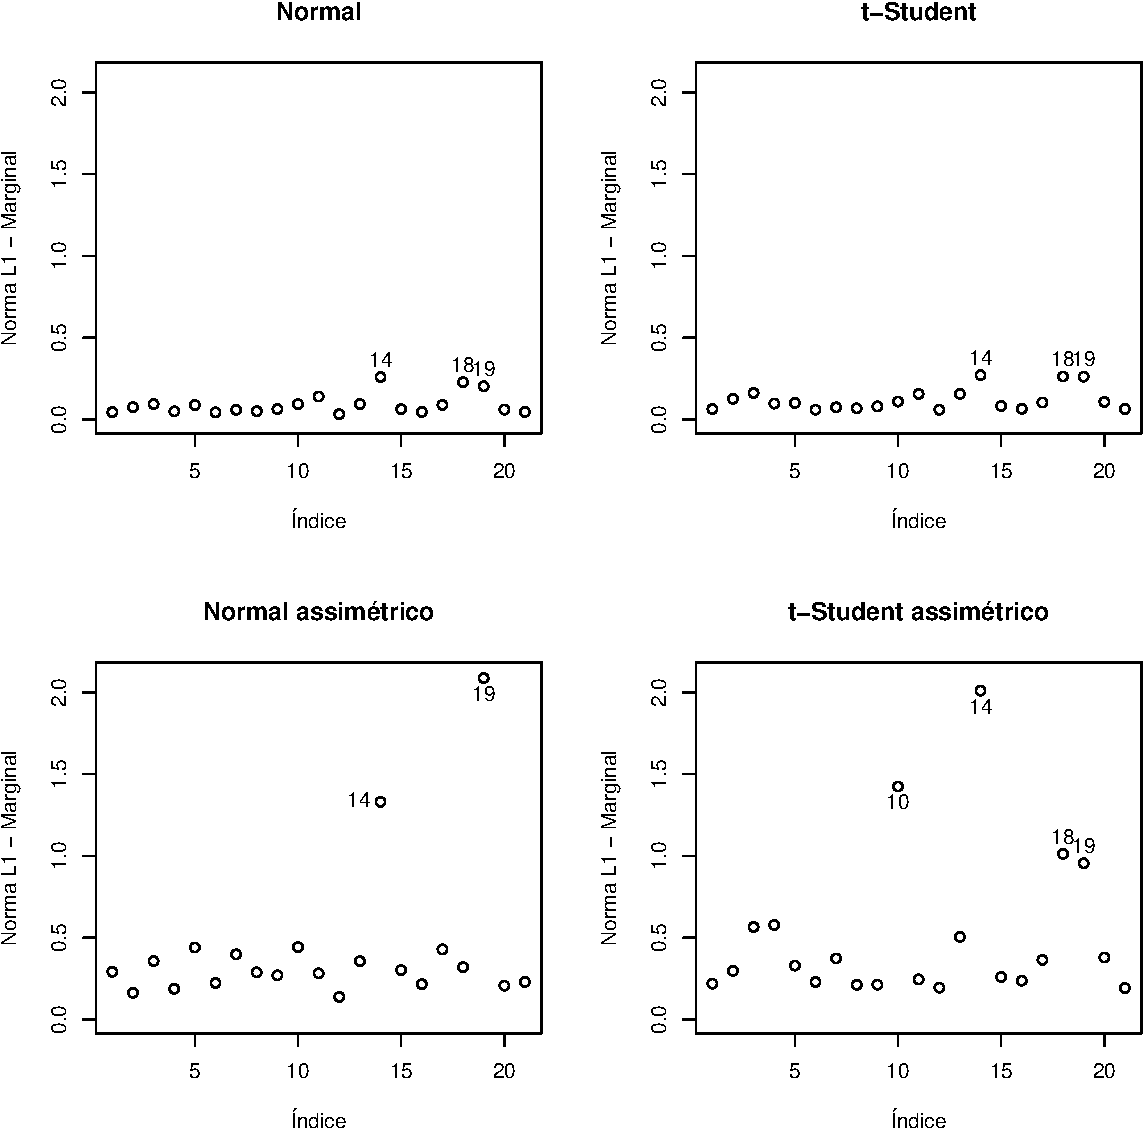
\includegraphics[width=\textwidth]{figuras/chap03_sec334_marg_l1.pdf}
\\ Fonte: Elaborada pelo autor.
\end{center}
\end{figure}

\begin{figure}[H]
\begin{center}
\caption{Influência marginal em $\betabf$ via divergência de Kullback-Leibler dos modelos contaminando as observações 14 e 19}
\label{fig:chap03_sec334_marg_kl}
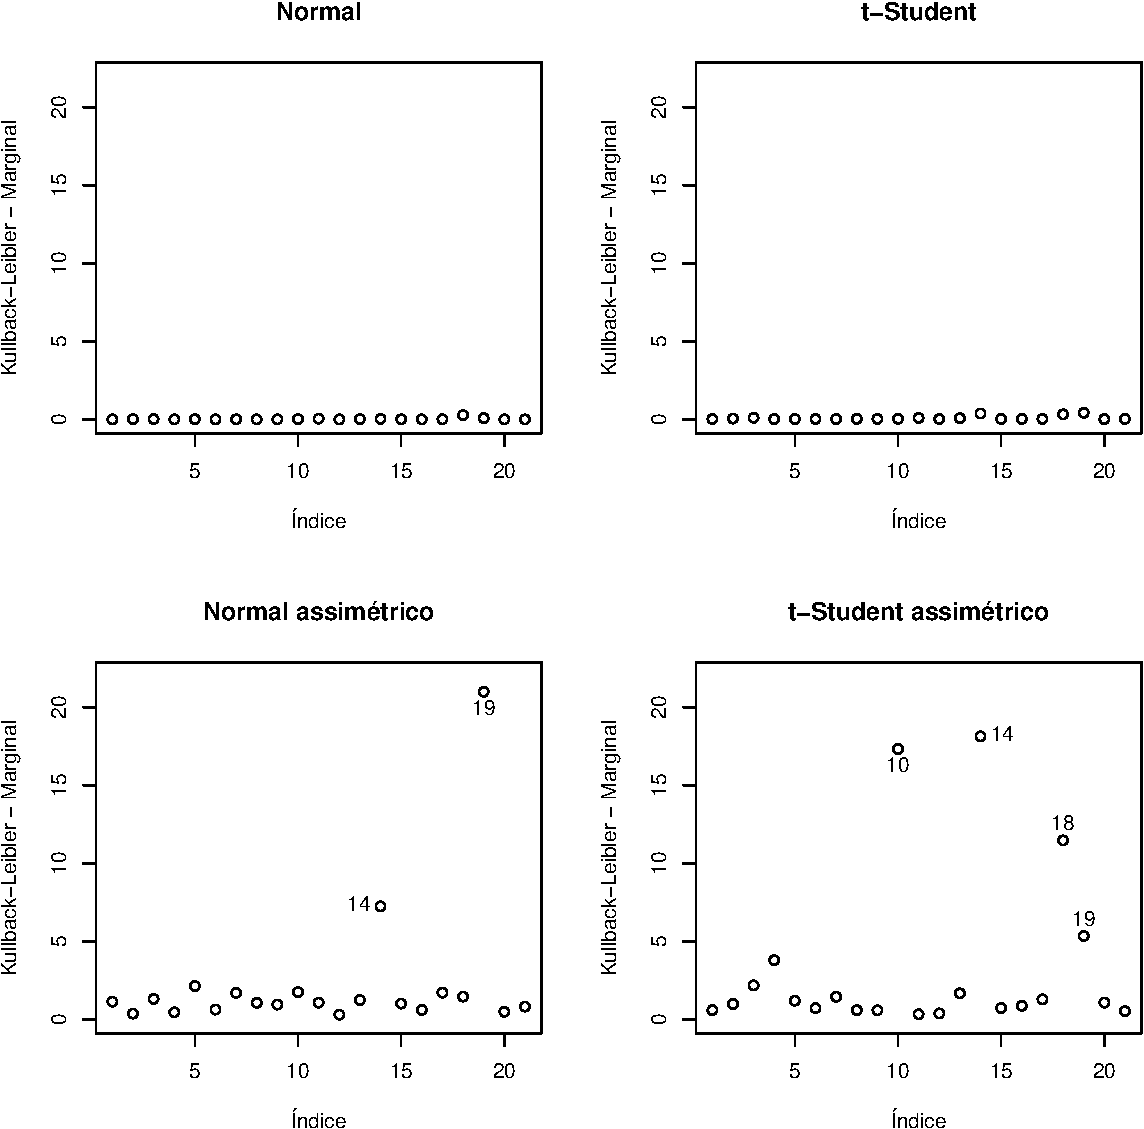
\includegraphics[width=\textwidth]{figuras/chap03_sec334_marg_kl.pdf}
\\ Fonte: Elaborada pelo autor.
\end{center}
\end{figure}